\documentclass[UKenglish]{uiomasterthesis}
\usepackage{caption}
\usepackage{booktabs}
\usepackage{algpseudocode}
\usepackage{algorithm}
\usepackage{graphicx} 
\usepackage[UKenglish]{uiomasterfp}
\usepackage[nottoc]{tocbibind}
\usepackage{amsmath}
\usepackage{amssymb}
\usepackage{amsfonts}
\usepackage{amsthm}
\usepackage{bm}
\usepackage{mathtools}
\usepackage{import}
\usepackage[hidelinks]{hyperref}
\usepackage[nohyperlinks]{acronym}
\usepackage[noabbrev,nameinlink]{cleveref}
\usepackage{tikz}
\usepackage{pgfplots} 
\usepackage{pgf} 

\usepackage[backend=biber, style=numeric-comp, sorting=none]{biblatex}
\addbibresource{ref.bib}
\usetikzlibrary{arrows, arrows.meta, positioning, calc}
\usepackage{listofitems}


\makeatletter
\AtBeginDocument
 {
   \def\ltx@label#1{\cref@label{#1}}%add braces
   \def\label@in@display@noarg#1{\cref@old@label@in@display{#1}}%remove braces
\def\label@in@mmeasure@noarg#1{%
    \begingroup%
      \measuring@false%
      \cref@old@label@in@display{#1}%remove braces for multline, see https://tex.stackexchange.com/q/737204/2388
    \endgroup}%  
 } %
\makeatother

\pgfplotsset{compat=1.18}

\def\mathdefault#1{#1}
\everymath=\expandafter{\the\everymath\displaystyle}

\title{Explainable Reinforcement Learning}
\subtitle{Discovering intent based explanations for heterogeneous cooperative multi agent reinforcement learning agents}
\author{Ada Hatland}
\date{August 2024}


\pagenumbering{roman}

\begin{document}

\uiomasterfp[master, program={Informatics: Robotics and Intelligent Systems},
  color=orange, dept={Department of Informatics}, fac={The Faculty of Mathematics and Natural Sciences},
  supervisors={Dr. Dennis Gro\ss \and Prof. Kyrre Glette\and Dr. Helge Spieker}, image = {images/cat.png}]

\renewcommand*\acffont{\textit}

\section*{Declaration of AI use}
In this thesis generative models have been used for topic suggestion, a small part of figure creation, equations and parts of the code used for creating plots, as well as debugging and documentation. All code suggested has been verified by a human. Generative models have \textbf{not} been used for text generation. I, the author, take full responsibility for the contents of this thesis.


\section*{Acknowledgments}
I would like to thank my external supervisor Dennis Gro\ss, as well as my internal supervisor Kyrre Glette for their guidance and support in writing this thesis. They have been of significant help when discussing how to proceed and what remains on the to-do list. I would also like to thank my cat Nokia for emotional support throughout the writing of this thesis.

\section*{Acronyms}
\begin{acronym}[ICANN]
    \acro  {rl}   [RL]   {Reinforcement Learning}
    \acro  {xrl} [XRL] {Explainable Reinforcement Learning}
    \acro  {xdrl} [XDRL] {Explainable Deep Reinforcement Learning}
    \acro  {ai}   [AI]   {Artificial Intelligence}
    \acro  {xai}  [XAI]  {Explainable Artificial Intelligence}
    \acro  {marl}  [MARL]  {Multi Agent Reinforcement Learning}
    \acro  {mdp}  [MDP]  {Markov Decision Process}
    \acro  {dqn}  [DQN]  {Deep Q-Network}
    \acro  {ppo}  [PPO]  {Proximal Policy Optimization}
    \acro  {drl}  [DRL]  {Deep Reinforcement Learning}
    \acro  {rnn}  [RNN]  {Recurrent Neural Network}
    \acro  {lstm}  [LSTM]  {Long Short Term Memory}
    \acro  {mbrl}  [MBRL]  {Model-Based Reinforcement Learning}
    \acro  {llm}  [LLM]  {Large Language Model}
    \acro  {ea}  [EA]  {Evolutionary Algorithm}
    \acro  {nsga}  [NSGA-II]  {Non-Dominated Sorting Genetic Algorithm II}
    \acro  {nn}  [NN]  {Neural Network}
    \acro  {aec}  [AEC]  {Agent Environment Cycle}
    \acro  {cnn}  [CNN]  {Convolutional Neural Network}
    \acro  {drc}  [DRC]  {Deep Repeated ConvLSTM}
    \acro  {pomdp}  [POMDP]  {Partially Observable Markov Decision Process}
\end{acronym}

\abstract
This is the abstract

\lefthyphenmin=1000
\tableofcontents
\listoftables
\listoffigures
\chapter{Introduction}

\pagenumbering{arabic}
Sequential decision-making problems are problems where one decision leads to a new state that requires a new decision to be made. An example of this is autonomously driving from point A to point B through city streets. For these types of problems \ac{rl} systems are used. \ac{rl}, both multi- and single-agent models have seen a significant rise in successful use and applicability in recent years, with models such as AlphaGo\cite{article} and smacv2\cite{ellis2023smacv2}. These models learn by agents performing actions in a given state decided by a policy that lead to a new state, and learning by receiving rewards depending on if the new state is preferable to the previous, the aim is to learn a near optimal policy for achieving a fixed goal\cite{Sutton1998}. The agent uses an observation of the state to choose an action. The environment describes how an action affects the state. See \cref{fig:rl_basics}. In a \ac{marl} system, we would have multiple agents.

\begin{figure}[H]
    \centering
    \hspace{-4cm}
    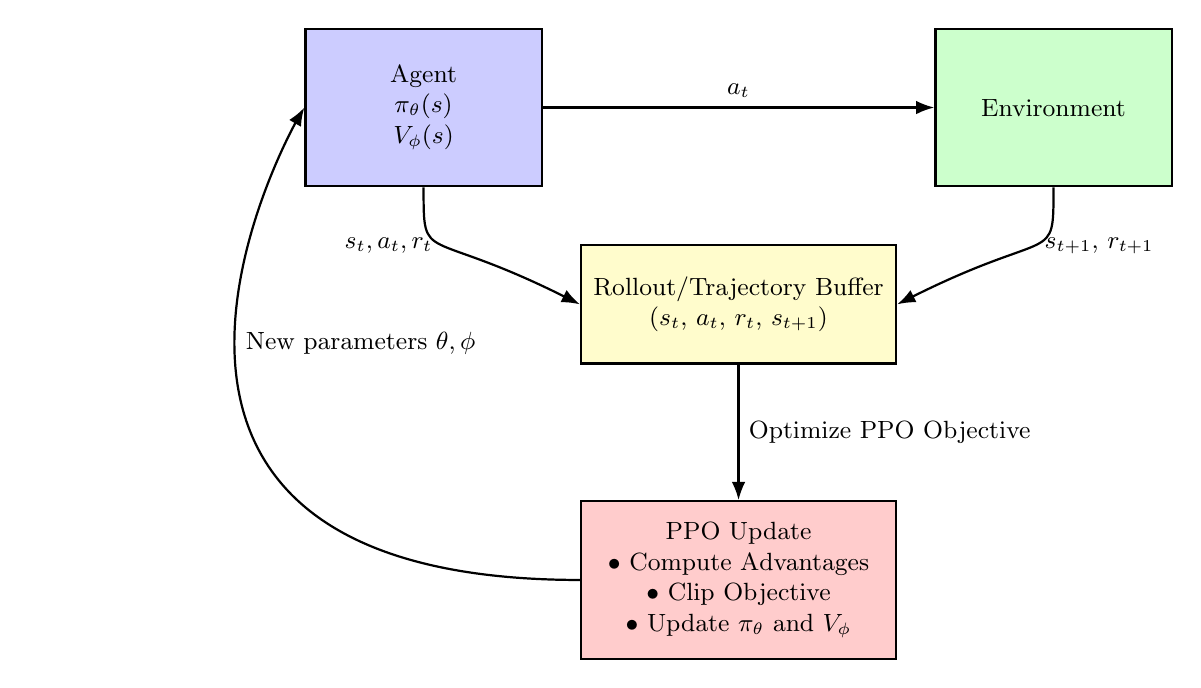
\begin{tikzpicture}[>=Latex, node distance=2.5cm, auto, font=\small]
    % Agent Node (with Policy and Value Networks)
    \node[draw, thick, rectangle, fill=blue!20, minimum width=3cm, minimum height=2cm, align=center] (agent)
    at (-4,3) {Agent \\ \(\pi_\theta(s)\) \\ \(V_\phi(s)\)};

    % Environment Node
    \node[draw, thick, rectangle, fill=green!20, minimum width=3cm, minimum height=2cm, align=center] (env)
    at (4,3) {Environment};

    % Arrow: Agent to Environment (Action)
    \draw[->, thick] (agent.east) -- node[above] {\(a_t\)} (env.west);

    % Rollout/Trajectory Buffer Node
    \node[draw, thick, rectangle, fill=yellow!20, minimum width=4cm, minimum height=1.5cm, align=center] (buffer)
    at (0,0.5) {Rollout/Trajectory Buffer \\ \((s_t,\, a_t,\, r_t,\, s_{t+1})\)};

    % Arrow: Environment to Rollout Buffer (State & Reward)
    \draw[->, thick] (env.south) .. controls +(0,-1) and +(2,1) .. node[right] {\(s_{t+1},\, r_{t+1}\)} (buffer.east);

    % Arrow: Agent to Rollout Buffer (State, Action, Reward)
    \draw[->, thick] (agent.south) .. controls +(0,-1) and +(-2,1) .. node[left] {\(s_t, a_t, r_t\)} (buffer.west);

    % PPO Update Node
    \node[draw, thick, rectangle, fill=red!20, minimum width=4cm, minimum height=2cm, align=center] (ppo)
    at (0,-3) {PPO Update \\ \(\bullet\) Compute Advantages \\ \(\bullet\) Clip Objective \\ \(\bullet\) Update \(\pi_\theta\) and \(V_\phi\)};

    % Arrow: Rollout Buffer to PPO Update
    \draw[->, thick] (buffer.south) -- node[right] {Optimize PPO Objective} (ppo.north);

    % Arrow: PPO Update to Agent (New Parameters)
    \draw[->, thick] (ppo.west) .. controls +(-7,0) and +(0,0) .. node[right] {New parameters \(\theta, \phi\)} (agent.west);
\end{tikzpicture}
\caption{Diagram showing the \ac{ppo} update algorithm}
\label{fig:rl_basics}
\end{figure}


\section{Motivation}
\label{sec:motivation}
A significant problem with many deep machine learning models, including \ac{marl} policies, is known as the black box problem\cite{zednik2019solving}. This problem describes how the processing of information is hidden from a human user due to the opacity of the model, and we just have to trust that the model uses relevant data to come to the conclusion it does, which it often doesn't do. For many tasks and models where the impact of the output isn't highly significant this isn't a big issue, but for tasks like autonomous driving we simply cannot use these models without trust for the models processing of data and that the solution given wont hurt anyone. We can considering autonomous driving as a \ac{marl} system if we consider each vehicle as an agent. To solve this we would like to have models that along with an output can provide us with some kind of reasoning for what information is used and how.

All this essentially means, until the black box problem is solved, autopilot will always require a driver behind the wheel\cite{tian2018deeptest}. Despite having high accuracy, precision and recall, a reinforcement learning model might choose a less than preferable action in edge cases or states not well covered by training and test sets, for example driving on snowy roads when all images in the training data is from warmer climates, or combinations that aren't well covered, like a foggy, snowy road with a sharp right turn.

With a way to ask the agent for intent, we could find that it has learned to always expect there to not be a car around the corner, which is not always obvious from looking at the dataset, but if it in a decision relies on the road to be empty to choose a safe route, this is obviously a huge issue. This paper aims to explain how an agent in a \ac{marl} setting decides on an action due to what it expects from other agents in the future. The field working on combating this issue is known is Explainable reinforcement learning.

\section{Problem statement}
\label{sec:problem}
The focus of this paper will be to rework and apply methods for general \ac{xai} to Reinforcement Learning, and expand on \ac{xrl} methods already developed. In particular we will focus on an agent and how the expected future states of other agents will affect it in its decision making process. The environment we will focus on is a \ac{marl} environment known as Knights Archers Zombies \cite{KAZ} made for Python. We use this because it is a cooperative environment where each agent has to consider other agents, both of the same type as itself, and other types. If we used an environment where all the agents are identical, our findings will be less useful for other environments where the agents aren't identical. In many real life scenarios agents will not be identical. If we once again consider autonomous vehicles, most vehicles are different in some way. A very obvious example of this is considering cars and motorcycles. Where because of their size difference, their paths chosen will often be different.

In psychology it is well known that most human based decisions are made with intent\cite{inbook}, and by focusing on the expectation of what future states will look like we can consider this the intent of the agent. If we are accurately able to extract the intent of an \ac{rl} policy we are better able to explain the choice made and we are more comfortable with trusting that the choice made is a good decision. Concretely we hypothesise that by analyzing expected future states and events we could find the intent of the agent, which we could use to ensure the agent acts in a safe or desirable manner. The main question we aim to answer is what information, found in weights or design of the policy, or information extracted by knowing the weights and design, is the most important for separate prediction models to be able to predict future states and actions, in cases where we do not have access to a decent world model, or such a model does not exist.


\section{Scope and limitations}
We aim to construct a framework to describe the intent of the agents in the KAZ environment, and we aim to make it applicable to other environments as well. However, due to time limitations we restrict the framework to only accept PettingZoo example environments or environments created with the PettingZoo environment creation tool. \ac{marl} environments can be divided into two major categories, \ac{aec} and parallel. \ac{aec} environments are environments where the state transition happens after each agent chooses an action, and parallel environments are environments where all the agents choose an action each before the transition happens. See \cref{fig:aec}.

Due to limited time and resources the size of policy or value networks, as well as any other \acp{nn} or otherwise computationally expensive algorithm used, will have to be significantly limited, this will impact results in a meaningful way, and therefore we will keep all \acp{nn} comparable sizes, and focus on doing experiments on how other factors than network size impact the results.

We do not have access to any real world datasets, so its hard to ensure the methods we have developed will be directly applicable, however the results we get will still be relevant for later research in the area.
\begin{figure}[H]
\centering
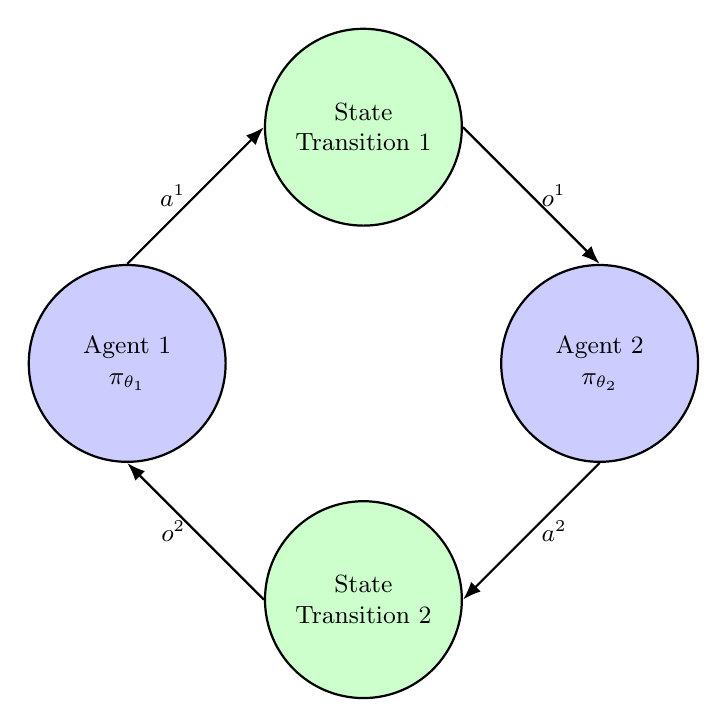
\begin{tikzpicture}[>=Latex, node distance=2.5cm, auto, font=\small]

    % Agent 1 Node
    \node[draw, thick, circle, fill=blue!20, minimum size=2.5cm, align=center] (agent1)
    at (-3,3) {Agent 1 \\ \(\pi_{\theta_1}\)};

    % Transition 1 Node
    \node[draw, thick, circle, fill=green!20, minimum size=2.5cm, align=center] (trans1)
    at (0,6) {State \\ Transition 1};

    % Agent 2 Node
    \node[draw, thick, circle, fill=blue!20, minimum size=2.5cm, align=center] (agent2)
    at (3,3) {Agent 2 \\ \(\pi_{\theta_2}\)};

    % Transition 2 Node
    \node[draw, thick, circle, fill=green!20, minimum size=2.5cm, align=center] (trans2)
    at (0,0) {State \\ Transition 2};

    % Arrows between nodes
    \draw[->, thick] (agent1.north) -- node[left] {\(a^1\)} (trans1.west);
    \draw[->, thick] (trans1.east) -- node[right] {\(o^1\)} (agent2.north);
    \draw[->, thick] (agent2.south) -- node[right] {\(a^2\)} (trans2.east);
    \draw[->, thick] (trans2.west) -- node[left] {\(o^2\)} (agent1.south);

\end{tikzpicture}

\caption{Example \ac{aec} in an environment with 2 agents.}
\label{fig:aec}
\end{figure}

\section{Research methods}
\label{sec:research}
This section describes the methods we use to answer the questions we have posed. The methodology mainly focuses on produced datasets made with a digital \ac{rl} environment, which does mean we have access to a world model, however as we want to answer the research questions without the use of a world model we will only be using the results of simulations to create our methods. The effect of this is that the methods will be compatible with \ac{rl} systems where we do not have access to a world model.

Producing our own dataset has the benefit of no restrictions, other than hardware restrictions, on the datasets size. We can also produce variations of these datasets by altering the simulations used to create them which would in a real world setting often be impossible, e.g. access to gradients during inference.

The datasets produced will be sets of full or partial trajectories in given environments along with other relevant data like integrated gradient, or Shapley values for the observations in the trajectories. We use these datasets to train predictive \acp{nn} with two main types. Event prediction, for example whether an agent encounters a critical state within the next 10 timesteps, which could represent a dangerous situation for an autonomous vehicle, and state prediction, which for example could be the x and y coordinates of a given agent 10 timesteps into the future.

We will first be focusing on including explanations for the observations and observe and analyze the effects on event and state predictors, then we will be using \ac{nn} policies with access to memory and include their representation of memory along with the observation, hidden values for lstm and once again observe and analyze effect on the predictors.

\section{Ethical considerations}
\ac{marl} is an important field in development for military purposes\cite{military_marl}, and while this research is not supposed to effectivize warfare its possible that it ends up being relevant for unintended areas of research, including but not limited to military use-cases. This is especially the case because I aim to develop methods for general \ac{marl} use and not a specific area of research, like medicine or sports. It is more or less impossible to restrict access to these methods for specific areas of research.

If this research aids to make \ac{marl} methods applicable to real world settings there is the possibility it risks increasing job displacement issues. This is an issue that affects most \ac{ai} research and can be mitigated by programs to reeducate people whose jobs it might affect, and increasing employment in developing and monitoring \ac{ai} tools.


\section{Main contributions}
As discussed in \cref{sec:motivation}, \cref{sec:problem} and \cref{sec:research}, there are certain specific objectives we aim to reach. In general we aim to expand on current future prediction research.

\begin{itemize}

    \item \textbf{Objective 1: Observation space}\\
        Most current methods assumes the observation space to be image based, and bases research on information found in convolutional layers, either regular \acp{cnn}, or convLSTM layers.

    \item \textbf{Objective 2: Feature importance as input}\\
        Using feature importance from the policy to improve future predictions is a novel idea, and has potential to improve future predictions by a significant margin.

    \item \textbf{Objective 3: Memory as input}\\
        Earlier research has found that including hidden states from the \ac{drc} architecture had a significant effect on accuracy when predicting future states and events. We aim to expand on this and use hidden states from \acp{lstm} layers and observe the effect and analyze how it differs from using the ConvLSTM hidden values.

\end{itemize}

\section{Thesis outline}
This thesis will be structured as follows:
\begin{itemize}

    \item \textbf{\cref{chap:background}: Background and related works}\\
        This chapter will introduce important concepts, both \ac{rl} and explainability related, and briefly discuss the history of \ac{xai} methods, and how they are applicable to my use case. We will also consider \ac{xrl} methods that are already developed and how to expand or integrate them into developed methods of our own.

    \item \textbf{\cref{chap:meth}: Methodology}\\
        This chapter discusses the specific principles, procedures and techniques used to conduct the \ac{xrl} research done in this thesis, to ensure that the results we get are valid and reliable.

    \item \textbf{\cref{chap:exp}: Experiments}\\
        This chapter details the setup, results and analysis of the specific experiments we use to evaluate the hypothesis and answer research questions based on certain evaluation metrics, and baseline comparisons.

    \item \textbf{\cref{chap:disc}: Discussion}\\
        This chapter will analyze the results of the experiments and discuss their implication for \ac{xrl} research. It will also contain the limitations of our work and briefly discuss how to expand on any research done.
\end{itemize}


\chapter{Background and Related Works}
\label{chap:background}
In this chapter I will introduce relevant concepts that are required to fully understand this thesis.

\section{Supervised learning}
Supervised learning is a core concept in machine learning. To do supervised learning you require labeled data. You have a dataset with training samples, each sample is an example of some data with an associated label. An example is an image of a stop sign, with the label "stop sign". This is an example of a classification problem. The classification model is trained by making predictions for each data sample, and then comparing the prediction to the label. The model improves by iteratively modifying internal values to reduce the difference between prediction and label. In the case with the image of a stop sign, the model could predict 0.7 stop sign as 70\% confidence that it is an image of a stop sign, making the difference 0.3 which it tries to reduce. If there was no stop sign in the image the error would instead be 0.7 and the model would try to reduce this by making other adjustments to the weights. The other main type of supervised learning is regression, which works similarly, but instead of a yes or no question it attempts to predict a continuous value. Like the speed of a car 10 seconds from now, measured in km per h.

The goal is to make a mapping function $f(X)=Y$ where $X$ is a set of input data, like an image, and $Y$ is a set of labels.

\subsection{Algorithms}
There are several algorithms that satisfy the supervised learning concept. Decision trees is an example. In a decision tree you have nodes with rules that branch out, and depending on the value of a feature depending on the rule you go down a branch. Once you reach a leaf node, you have your decision. An example of a node is is there a strong prediction sign in this picture, which would lead to branches yes or no, and if you do not have a strong prediction you can conclude that the image does not contain a "stop sign", which would be the leaf node.

Another common type algorithm that this thesis will focus on is \acp{nn}. While decision trees are interpretable, \acp{nn} are not.

\subsection{Overfitting}
An issue that often arises when working with supervised learning is whats known as overfitting. This is when the model learns the training dataset too well, and doesnt capture to generalize between samples and labels, but rather the noise in the samples, which often dont represent a true correlation, i.e. a correlation that exists in the training dataset but not in the real world. This negatively affects the performance for the model on new data. To combat this, especially when training \acp{nn} which have a tendency to overfit, it is important with large and representative datasets.

Large and representative datasets are often costly to create. In this thesis however, we automatically create all required datasets, which means we do not face this issue, as both datasets used for training and testing the model are drawn from the same distribution, so any findings are not a result of skewed datasets. The only issue we could face is not creating a large enough dataset, which I circumvent by making it what is more than likely larger than necessary. 

\section{Reinforcement Learning Fundamentals}
To make sure all methods are understood well its important to make sure we have a proper understanding of the fundamentals of \ac{rl}, especially \ac{drl} and \ac{marl}. This section will go over the basics needed. \ac{rl} is not a supervised learning algorithm.


\subsection{Markov Decision Process in Reinforcement Learning}

A \ac{mdp} is a framework used to model decision-making in stochastic environments, like we want to in an \ac{rl} task. It is defined by a tuple with 5 elements:

$$\mathcal{M} = (\mathcal{S}, \mathcal{A}, P, R, \gamma)$$

where \(\mathcal{S}\) is the set of possible states, \(\mathcal{A}\) is the set of possible actions, \(P(s' | s, a)\) is the transition probability function, which defines the probability of moving to state \(s'\) when action \(a\) is taken in state \(s\), \(R(s, a, s')\) is the reward function that provides a reward for transitioning from state \(s\) to \(s'\) via action \(a\), \(\gamma \in [0,1]\) is the discount factor that determines the importance of future rewards.

The objective in an \ac{mdp} is to find a policy \(\pi(s)\) that maximizes the expected cumulative reward:

$$V^\pi(s) = \mathbb{E} \left[ \sum_{t=0}^{\infty} \gamma^t R(s_t, a_t, s_{t+1}) \mid \pi \right]$$

where \(V^\pi(s)\) is the value function that represents the expected return starting from state \(s\) and following policy \(\pi\). See \cref{fig:rl_basics}.


\subsection{Markov Decision Process in Multi Agent Reinforcement Learning}
In a \ac{marl} setting agents could have shared or independent \acp{mdp} depending on architecture. There are three main branches of \ac{marl}, cooperative, competitive and mixed. Our focus will be on cooperative \ac{marl}.
In a cooperative \ac{marl} setting the goal is some social welfare function that maximises rewards for the agents, either collective rewards or a mix of collective and individual rewards. In such a setting each agent has \ac{mdp}. Assuming that state space \(\mathcal{S}\) and discount factor \(\gamma\) is shared, which they will be in all my experiments, if two agents have the same reward structure $R$ and action space \(\mathcal{A}\) their objective would be the same, in which case they could share policy \(\pi\) and could therefore share \(\mathcal{M}\).

\subsection{Deep Reinforcement Learning}
Traditional RL methods struggle with scalability due to the fact that they rely on discrete state representations. \ac{drl} uses deep \acp{nn} to approximate the policy function $\pi_\theta(s)$, the value function $V_\phi(s)$, or the Q-function $Q_\theta(s,a)$, making it possible to represent these functions in continuous and complex environments. See \cref{fig:neural_network}. Input layer is size of state for all three functions. Output layer is size of action space for $Q_\theta(s,a)$ and $\pi_\theta(s)$. $V_\phi(s)$ only has one output node. In a feed forward \ac{nn} like we have here each node has the value of some activation function $\phi(x)$ where $x$ is the sum of nodes of the previous layer multiplied by their respective weights, usually as well as adding some bias, shown as the connections between the nodes. Common activation functions are $ReLU(x) = max(0,v)$ and $tanh=\frac{e^v-e^v}{e^v+e^v}$ where $v$ is the value before activation.
\begin{figure}[H]
    \centering
    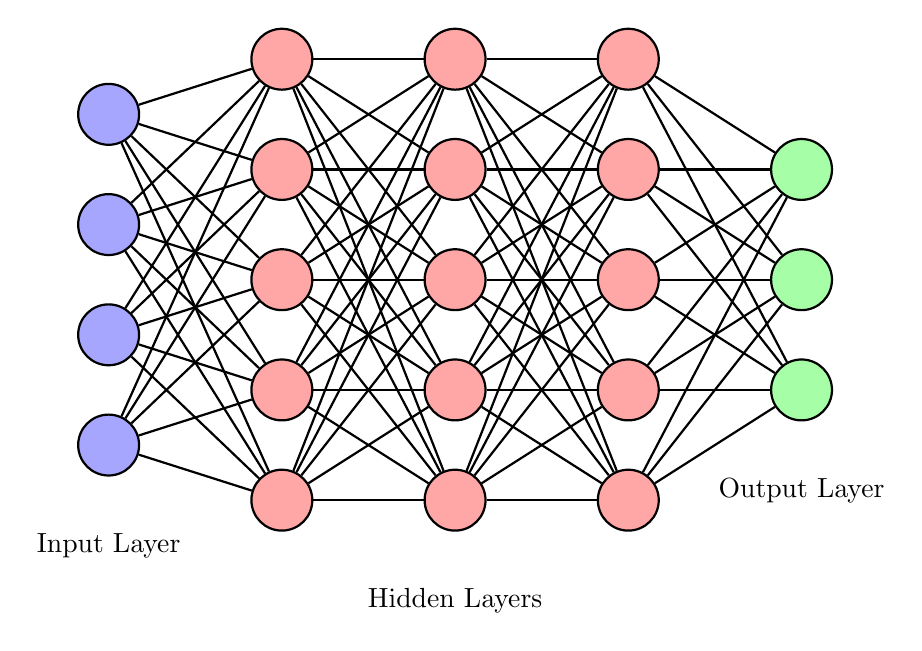
\begin{tikzpicture}[
        x=2.2cm, y=1.4cm, 
        mynode/.style={thick, draw=black, circle, minimum size=22}, % Base style
        inputnode/.style={mynode, fill=blue!35},  % Input layer
        hiddennode/.style={mynode, fill=red!35}, % Hidden layers
        outputnode/.style={mynode, fill=green!35} % Output layer
    ]
    
    \readlist\Nnod{4,5,5,5,3} % Number of nodes per layer
    
    \foreachitem \N \in \Nnod{ % Loop over layers
        \foreach \i [evaluate={\x=\Ncnt; \y=\N/2-\i+0.5; \prev=int(\Ncnt-1);}] in {1,...,\N}{ 
            
            % Choose color based on layer type
            \ifnum\Ncnt=1
                \node[inputnode] (N\Ncnt-\i) at (\x,\y) {}; % Input layer
            \else
                \ifnum\Ncnt=\Nnodlen
                    \node[outputnode] (N\Ncnt-\i) at (\x,\y) {}; % Output layer
                \else
                    \node[hiddennode] (N\Ncnt-\i) at (\x,\y) {}; % Hidden layer
                \fi
            \fi
            
            % Connect to previous layer
            \ifnum\Ncnt>1  
                \foreach \j in {1,...,\Nnod[\prev]}{ 
                    \draw[thick] (N\prev-\j) -- (N\Ncnt-\i); 
                }
            \fi 
        }
    }
    
    \node[align=center, below=1] at (N1-4.90) {Input Layer};
    \node[align=center, below=1] at (N3-5.90) {Hidden Layers};
    \node[align=center, below=1] at (N5-3.90) {Output Layer};
    \end{tikzpicture}
    \caption{Illustration of an example of a \ac{nn} with three hidden layers}
    \label{fig:neural_network}
\end{figure}


\subsection{Model-Free vs. Model-Based Reinforcement Learning}
Model-based and model-free reinforcement learning differ in how they represent environment transitions. In model-based reinforcement learning, the agent learns or has access to a model of the environment, which includes a transition function \( P(s' | s, a) \) and a reward function \( R(s, a) \) that determines the expected reward for taking action \( a \) in state \( s \) \cite{moerland2022modelbasedreinforcementlearningsurvey}. This allows the agent to simulate future outcomes without taking actions in the real environment. As a result, model-based methods are able to update policies based on imagined rollouts, which increases learning speed compared to executing the real environment transitions. Examples of model-based algorithms are Dyna\cite{10.1145/122344.122377} and DreamerV3\cite{hafner2024masteringdiversedomainsworld}.

In contrast, model-free reinforcement learning does not learn or utilize an explicit model of the environment. Instead, the agent learns by interacting directly with the environment and updating its network weights based on observed rewards. This approach is generally less sample-efficient but is applicable to environments where modeling the transition dynamics isn't feasible. Examples of model-free algorithms include Q-learning, \ac{dqn} \cite{mnih2013playingatarideepreinforcement}, and \ac{ppo} \cite{schulman2017proximalpolicyoptimizationalgorithms}.

Model-based methods enable explicit planning by using the learned environment transitions in methods such as Monte Carlo Tree Search \cite{_wiechowski_2022}, while model-free methods rely on direct experience to optimize behavior. We will be using \ac{ppo} to optimize our algorithms, and will not be using simulations or any other form of explicit planning, ensuring that the methods developed will be applicable in the most amount of environments.

\subsection{Recurrency in Deep Reinforcement Learning Policies}
Recurrency in \ac{nn} is a way to carry over information from previous timesteps to current ones, if we believe that information could be useful. \acp{rnn} are sometimes used when constructing the architecture of \ac{drl} policies \cite{hausknecht2017deeprecurrentqlearningpartially}, mainly for two reasons. The first one is for when your environment can be modeled as a \ac{pomdp}, in which case memory is important as the current observation is not always enough to capture all the information an agent could have. The second reason is for planning, like in the \ac{drc} architecture\cite{guez2019investigationmodelfreeplanning}. See \cref{fig:rnn}.

\begin{figure}[H]
    \centering
    \hspace{3.5cm}
    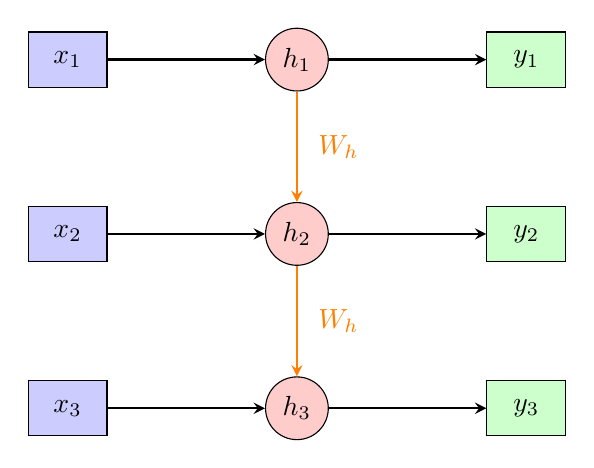
\begin{tikzpicture}[>=stealth, auto, node distance=1.5cm and 2cm]

    \begin{scope}[shift={(4,0)}, rotate=90]
  
    % Time step 1
    \node (x1) [draw, rectangle, fill=blue!20, minimum width=1cm, minimum height=0.7cm] {$x_1$};
    \node (h1) [draw, circle, fill=red!20, right=of x1] {$h_1$};
    \node (y1) [draw, rectangle, fill=green!20, right=of h1, minimum width=1cm, minimum height=0.7cm] {$y_1$};

    % Time step 2
    \node (x2) [draw, rectangle, fill=blue!20, below=of x1, minimum width=1cm, minimum height=0.7cm] {$x_2$};
    \node (h2) [draw, circle, fill=red!20, right=of x2] {$h_2$};
    \node (y2) [draw, rectangle, fill=green!20, right=of h2, minimum width=1cm, minimum height=0.7cm] {$y_2$};

    % Time step 3
    \node (x3) [draw, rectangle, fill=blue!20, below=of x2, minimum width=1cm, minimum height=0.7cm] {$x_3$};
    \node (h3) [draw, circle, fill=red!20, right=of x3] {$h_3$};
    \node (y3) [draw, rectangle, fill=green!20, right=of h3, minimum width=1cm, minimum height=0.7cm] {$y_3$};

    % Forward connections within each time step (black)
    \draw[->, thick, black] (x1) -- (h1);
    \draw[->, thick, black] (h1) -- (y1);
  
    \draw[->, thick, black] (x2) -- (h2);
    \draw[->, thick, black] (h2) -- (y2);
  
    \draw[->, thick, black] (x3) -- (h3);
    \draw[->, thick, black] (h3) -- (y3);

    % Recurrent connections between hidden states (orange)
    \draw[->, thick, orange] (h1) -- (h2) node[midway, right=4pt] {$W_h$};
    \draw[->, thick, orange] (h2) -- (h3) node[midway, right=4pt] {$W_h$};
    \end{scope}
\end{tikzpicture}
\caption{Recurrent neural network showing a 3 step time series with hidden values propagating through time.}
\label{fig:rnn}
\end{figure}

\subsection{Backpropagation and gradient descent}
Backpropagation is a training algorithm used to train \acp{dnn} to minimize error. If a network is differentiable you can use backpropagation. First you do a forward pass through the network, i.e. your network calculates a prediction based on an input. Then you calculate loss, the difference between true value and predicted value is passed to some function. MSE is one such function.
\[
\text{MSE} = \frac{1}{n} \sum_{i=1}^{n} (y_i - \hat{y}_i)^2
\]
Where $y$ is true value, $\hat{y}$ is predicted value, $n$ is amount of samples multiplied by outputs. If you are trying to predict $(x,y)$ coordinates, you would have two outputs, if you're trying to predict $x,y$ coordinates in 5 cases you would have $n = 10$.
Then you do a backwards pass, calculating loss with respect to the weights in the network using the chain rule. Then using gradient descent you change the weights to reduce loss.


\section{Approaches to Explainability in Reinforcement Learning}
\subsection{Post Hoc vs. Intrinsically Explainable Models}
This section will discuss benefits and drawbacks of explainable models divided into two main categories, Post hoc models and intrinsically explainable models.

Post hoc explainability refers to finding ways to understand already trained models. Instances where this doesn't pose more of a challenge can often be more efficient as you do not need to construct and train a model, which could often pose an issue both considering time spent and accuracy of the model. Making a model explainable only makes sense if we know it usually makes sensible decisions. There are however issues with making post hoc models.

\subsubsection{Temporal Aspect}
\ac{rl} policies all have a temporal aspect, which means several different actions over a certain period of time might contribute to a singular outcome, this could make it very challenging to pinpoint which actions were made for which outcome, especially if the outcome happens several states after the initial decision was made.

\subsubsection{Nature of Black Box Models}
Many \ac{rl} policies, especially deep \ac{rl} policies, which are the policies we will be working with, have complex inner connections due to the hierarchical structure of learning features in the input, sequences of non linear connections that are very hard to understand without spending a lot of time studying the specific connections learned by a model. It's often very difficult to accurately pinpoint the purpose of a node, especially because we do not know if it even has a purpose at all or it could have a lot of different purposes. Especially in environments with complex observation spaces.


\subsubsection{Lack of Transparency}
Tracing how an observation leads to a state, through the action chosen and the environment, is often challenging in models constructed without this in mind. If we do not know the processing of information of a model it's very hard to explain the rationalisation of an agent.

\subsubsection{Intrinsically Explainable Models}
Intrinsically explainable models have the already stated drawback of relying on careful model construction, which can be challenging and may impact model performance. While these models offer transparency from the get go, they are often less flexible and might not achieve the same level of accuracy as more complex \ac{rl} models. Given that we aim to analyze and compare already trained \ac{rl} policies, we will mostly focus on post hoc explainability methods in this thesis.



\subsection{Fidelity of Explainable Artificial Intelligence Methods}
It is important to understand why the current \ac{xai} methods not meant for \ac{rl} applications aren't always useful to us.

\ac{xai} methods not intended for reinforcement learning often provide explanations that don't necessarily represent the inner workings of an \ac{rl} policy, because an \ac{rl} policy has a temporal aspect as well. Broadly these methods can be categorised as feature-based explainers, and they often struggle to fully explain an agents behaviour or specific actions because they cannot capture the future view of an \ac{rl} policy. 

Saliency maps which have been successfully used for classification of images provide explanations about what part of the input was important for the outcome, which is highly relevant for classification tasks, but using the same method for an \ac{rl} policy doesn't sufficiently explain the intent of the agent\cite{atrey2020exploratory}.

Another commonly used \ac{xai} method is model distillation, which works by transferring knowledge from a large model to a smaller, usually interpretable, one, for instance a deep learning network to a decision tree \cite{bastani2019verifiable}. This has use cases in verifyability, but struggles to fully explain the temporal aspect of \ac{rl} policies, and are therefore not sufficient as an explainer.

However, these methods might still prove insightful in conjunction with other intent-based methods, the state in which a decision is made is obviously very relevant to why that particular decision was made. We could perhaps use these methods to answer questions such as "What part of agent As Observation this state, lead it to believe agent B would end up at these coordinates at a later state?"


\subsection{Future-Based Explanations}
Next, I will describe in slightly more detail, what is meant by an intent based explainer, like I want to develop, and how to use it.

\subsubsection{Design}
"Towards Future-Based Explanations for Deep RL Network Controllers"\cite{10.1145/3626570.3626607} broadly describes future-based intrinsically explainable methods. Future-based intrinsically explainable methods for \ac{drl} policies often take three inputs, the trajectories experienced by an agent, the environment and the agent. Then, they collect the rewards and interactions and use this information to train an explainer.

During inference, we can then apply the explainer to a state and action to get the expected future consequences of that action. Depending on the architecture we could either get the expected future consequence of any action, or just the one the agent decides on.

\subsubsection{Use Cases}
Designing a \ac{drl} solution requires choosing features in the observation, hyperparameter tuning, policy design and reward function among other things. This is a time, and resource, consuming process. These are usually picked by trial-and-error but could be made easier with assistance from an explainer.

Another, and perhaps more important, use case is safety. If when online, i.e. the chosen action will actually affect the state, we are expecting high likelihood of an unsafe state, we could instead of opting for the chosen action fall back to a known safe action, that could have a lower expected return, i.e. breaking instead of turning a corner if we have limited vision around the corner.


\subsubsection{Definition of Intent}
We define the state transition function $T(s, \textbf{a}, s')$ where $\textbf{a}$ is the set of simultaneous actions made by the set of active agents, in our case, one action per agent. Given $T$ the agent should when prompted output a set of trajectories $\tau = \{(s_0,\textbf{a}_0),(s,\textbf{a}),(s_1,\textbf{a}_1)...(s_n,\textbf{a}_n)\}$ where $s_0$ is the current state, $\textbf{a}_i$ is the set of actions taken in $s_i$, and $s_{i+1}$ is the state reached by $T(s_i,\textbf{a}_i, s_{i+1})$. We will apply a series of methods on $\tau$ to extract intent. One of these methods is discovering counterfactual trajectories, $'\tau$, where the actions made by the agents in $'\tau$ are as similar as possible to the actions made by the agents in $\tau$, but the total reward gained is as low as possible. $'s_0 = s_0$ and given an identical transition function $T$ the goal is to discover which actions are most important to receive the reward. This method is similar to and inspired by ACTER\cite{gajcin2024acter}, see \cref{sec:acter}.

\section{Explainable Deep Reinforcement Learning: State of the Art and Challenges}
This paper is a comprehensive survey of the most common state of the art methods applicable to \ac{rl}. Section 4 specifically highlights \ac{xdrl} methods. This subsection will focus on these methods\cite{sota}. This section will serve to give an overview of \ac{xrl} methods that already exist, and if and how I use these methods to develop my own.

\subsection{Feature importance}


\subsubsection{LIME and SP-LIME}
LIME and SP-LIME are model-agnostic methods that explain chosen actions in specific states by slightly modifying input features and fitting an interpretable linear surrogate model that approximates the behaviour of the model locally. SP-LIME selects a representative set of these explanations to create a global explanation for how the model selects an action. These methods explain what features are important when deciding on an action in a given state.

\subsubsection{Shapley Additive exPlanations}
Shapley values is a method of computing marginal contributions from cooperative game theory. It assigns a Shapley value to each feature which is the mean of that features marginal contribution over all combinations of features to establish a fair attribution of credit to each player, or feature in the case of machine learning. This method is very computationally expensive and as such, approximations of this method are used instead.

\subsubsection{Layer-wise Relevancy Propagation}
LRP is a method to assign importance to each node in the network by working backwards from the output to the input. It looks at what nodes in the last hidden layer influenced the output and redistributes prediction scores to these nodes, it then looks at what nodes in the layer before influenced the nodes in the last hidden layer, until you have a complete map of how the network nodes affected each other to produce the output. This method helps reveal hidden patterns in model behaviour.

\subsection{Policy explanations}

\subsubsection{HIGHLIGHTS}
This is a intrinsically explainable \ac{rl} algorithm and it works by extracting sub-trajectories with important states, states where a wrong action can lead to significant decreases in reward, to explain how the agent acts in these states. It also provides context in the form of neighbouring states in the important sub-trajectories, in order for users to understand why it chose the trajectory it did.

% \subsection{Objective explanations}

% \subsection{Outcome explanation}


\section{Relevant Methods}
There are several papers written on \ac{xai} and \ac{xrl} problems. Milani et al.\cite{milani2022survey} categorise \ac{xrl} into three main categories, feature importance (FI), learning process and \ac{mdp} (LPM) and Policy-level (PL). FI considers the immediate context for actions, i.e. what part of the input was important for a single action, LPM considers techniques that highlight which experiences in training were influential for the final policy and PL focuses on long term effects and behaviour. Since we are interested in future states and actions we will look at influential trajectories and transitions within these trajectories. It is important to view these transitions in the context of the trajectory to understand the long term effects and not just immediate, which are of less interest in this paper, if we find the state with a high state importance $I(s)$, $I(s) = max_aQ(s,a)-min_aQ(s,a)$ most similar by some similarity measure to an arbitrary current state we could find the resulting trajectory and expect the agent to intend a similar outcome. There are also ways to convert \ac{rnn} policies to an interpretable models post-hoc, which might be relevant if we use an \ac{rnn}. This paper will explore PL explainability further.

In particular "What did you think would happen? Explaining Agent Behaviour through Intended Outcomes" \cite{yau2020did}, "Explainable Reinforcement Learning via a Causal world model" \cite{yu2024explainable} and "CrystalBox: Future-based explanations for input-driven deep \ac{rl} systems" \cite{patel2024crystalbox} are highly relevant due to the fact that they all describe temporal connections between current actions and future states or actions.

"Are large language models post-hoc explainers" \cite{kroeger2024large} Could be relevant as using other explainers to compare explanations is useful. "ACTER: Diverse and Actionable Counterfactual Sequences for Explaining and Diagnosing \ac{rl} Policies" \cite{gajcin2024acter} 

\subsection{What did you think would happen? Explaining Agent Behaviour through Intended Outcomes}
What did you think would happen describes what an agent expects to happen in future states, and why the current action is chosen based on the future expectations. As stated in the paper, a limitation of their method means it doesn't work well with high dimensionality. The two main difference between this paper and the problem i aim to solve is that they're focusing on an environment with a single agent and that our observation space will be high dimensionality. It uses Q-learning and Markov-chains that train simultaneously with a "belief map" that shows what the agent expects the environment to look like in future states. In the simple examples used in the paper it shows where it believes the taxi should drive and therefore chooses an action to follow this path. This is not directly applicable to my thesis as it's unlikely that Q-learning or Markov chains will be viable for the policy and explainer based on the environment. However the paper is successful in explaining an agents underlying motivations and beliefs about the causal nature of the environment, and using similar methods might be an effective means for making \ac{marl} agents with higher dimensionality understandable from a human perspective. 

\subsection{Explainable Reinforcement Learning via a Causal world model}
Explainable Reinforcement Learning via a Causal world model constructs a sparse model to connect causal relationships, without prior knowledge of the causal relationship, rather than a fully connected one, but they still achieve high accuracy and results comparable to other fully connected \ac{mbrl} policies. Which is important, as there is often a trade off between explainability and performance. Using the same model for both explanations and choosing actions also make the explanations faithful to the intentions of the agent. The paper also describes a novel approach to derive causal chains from the causal influence of the actions, which lets us find the intent of the agent. The paper is successful being applied to \ac{mbrl}, and is also applicable to models with infinite actions spaces, which is a limitation of some other models, see previous sub section.

A limitation of the paper is that it requires a known factorisation of the environment, denoted by $\langle S, A, O, R, P, T, \gamma \rangle$, where S is state space, A is action space, O is observation space, R is reward function, P is probability function for the probability of transitioning from state $s$ to state $s'$ given action $a$, T is the termination condition given the transition tuple $(s,a,o,s')$, and $\gamma$ is the discount factor. Considering we will be working with hand crafted simulations we will have access to all of these, however its not certain that if we depend on this method that our contributions will be applicable to certain other environments where the factorisation is not known.


\subsection{CrystalBox: Future-Based Explanations for Input-Driven Deep Reinforcement Learning Systems}
CrystalBox introduces a model-agnostic, post-hoc, future based explanation for \ac{drl}. It doesn't require altering the controller, and works by decomposing the future rewards into its individual components. While this isn't exactly the kind of explanation we are looking for, it could be a great tool in developing an explainer that considers other agents actions in a multi agent cooperative environment, which is the goal of our paper, because it is post-hoc, and easily deployable. Especially because it was constructed for input-driven environments. The original paper claims it offers high fidelity solutions for both discrete and continuous action spaces. KAZ has a discrete action space but we might do some work with other environments as well.

It's not certain to be useful because it works by decomposing the reward function, and it's not safe to assume the reward function will even be useful to decompose.


\subsection{Are Large Language Models Post Hoc Explainers}
A \ac{llm} is a predictive model that generates text based on a prompt you give it, be it continuing the prompt or responding, and can often give the impression of comprehension of human language and a deeper understanding of the topic at hand.  The paper aims to investigate the question "Can LLMs explain the behaviour of other complex predictive models?" by exploiting the in-context learning (ICL) capabilities of \acp{llm}. ICL allows \acp{llm} to perform well on new tasks by using a few task samples in the prompt. A benefit of using an \ac{llm} as a post-hoc explainer, is that the output given by the model will already be written in natural language and should be understandable by a layman. The paper presumes that the local behaviour of a model is a linear decision boundary, and by using a sample x and perturbing it to x', and presenting both the samples and the perturbation as natural language we could get an explanation from the \ac{llm} for the outcome. With a sufficient number of perturbations in a neighbourhood around x the \ac{llm} is expected to explain the behaviour in this neighbourhood, and rank the features in order of importance.

While the faithfulness of the \ac{llm} as an explainer is on par with other \ac{xai} methods used for classification, meaning that the reasons provided are enough to explain the output, I am sceptical of the fidelity of the \ac{llm} for two reasons. One is the same as for why other \ac{xai} models often struggle with fidelity, the temporal aspect. If applied in the same way as in the paper it would not consider the intent or the past and only what part of the current observation made it make a certain decision. The other is that I am sceptical of claims presented by an \ac{llm} in general as these are all just guesses. Good guesses a lot of the time, but still just guesses. 

We could however potentially change the implementation so it considers the temporal aspect, and this might be a viable post hoc explainer after some more research into prompt engineering.


\subsection{ACTER: Diverse and Actionable Counterfactual Sequences for Explaining and Diagnosing Reinforcement Learning Policies}
\label{sec:acter}
The paper presents ACTER, an algorithm that uses counterfactual sequences with actionable advice on how to avoid failure for an \ac{rl} policy. It does this by using an \ac{ea} known as \ac{nsga} to generate counterfactual sequences that don't lead to failure as close as possible to factual sequences that lead to failure. This paper presents counterfactual sequences and not just actions, which means it also presents how to avoid the state that lead to failure to begin with, which should, if ACTER is implemented correctly, allow us to significantly reduce the amount of times our policy fails. It also offers multiple counterfactuals to allow the end user to decide which counterfactual is preferable to their use case.

There are 4 hypothesises tested by the paper. The last two considers laymen users and are therefore not as interesting to us. The first two however "ACTER can produce counterfactual sequences that prevent failure with lower effort and higher certainty in stochastic environments compared to the baselines." and "ACTER can produce a set of counterfactual sequences that offer more diverse ways of preventing failure compared to the baselines." are partially and fully confirmed respectively. Which means ACTER will likely be a useful tool to explain and diagnose our \ac{rl} policy.


\section{Related Works}
This section describes recent development in the field of planning and future predictions. All the papers described here are directly relevant to the methods i developed.

\subsection{Predicting Future Actions Of Reinforcement Learning Agents}
\label{sec:predicting_actions}
This paper describes a method developed by the author that predicts future actions and events \cite{chung2024predictingfutureactionsreinforcement}. It does this for non planning policies, like Impala, implicit planning policies like \ac{drc}, see \cref{sec:impl_planning}, and explicit planning policies like MuZero and Thinker.

Non planning policies are policies designed without planning in mind. Pure \ac{nn} policies without recurrency are considered to be non planning, as they have not been found to exhibit planning like behaviour. This paper found that when predicting future states and actions both inner states from implicit planners, and explicit planners improved accuracy over non planning agents.

Explicit planners are agents who simulate future states with a world model before making a decision on what action to take. They rely on the world model being accurate, and so does using them to predict future states and actions. In some environments learning an accurate world model is not feasible, an example of this is autonomous driving.

The paper proposes two methods on predicting future states and actions, simulation based and inner state based. The inner state approach is most effective when working with explicit planners, but also shows significant improvement for implicit planner agents. The simulation based approach performs very well on implicit planner agents, but requires the opportunity to train a decently performing world model. The paper also shows with an ablated world model, the inner state approach performs better.

\subsection{An Investigation of Model Free Planning}
\label{sec:impl_planning}
This paper investigates whether planning like behaviour can emerge from model free \ac{rl}, without any explicit planning methods or inductive biases designed to induce planning behaviour \cite{guez2019investigationmodelfreeplanning}. The authors introduce and explore if the \ac{drc} architecture can learn to implicitly plan through training. World models suffer from scalability issues, and inductive biases require a priori knowledge of the environment. The \ac{drc} architecture is comprised of $3$ layers of ConvLSTMs and each layer is iterated through $3$ times each at each timestep.

This architecture is tested on domains that require planning such as Sokoban, and they test the agents ability to generalize as well as data efficiency. The results of the paper is that not only does the model exhibit planning like behaviour, but it outperforms state of the art methods that use inductive biases or world models. The paper described in \cref{sec:predicting_actions} finds that using the inner state of implicit planner agents improves predicted future states and actions.


\chapter{Methodology}
\label{chap:meth}
This chapter will elaborate on the methods I will use to perform the experiments. Firstly, in \cref{sec:event_state_meth}, I will discuss in detail the state and events we want to predict. Then, in \cref{sec:feat_imp_meth}, I will elucidate how i attribute importance to observation features. After that, in \cref{sec:intent_meth}, I will define what I mean by intent for an agent in a \ac{rl} setting. Then, in \cref{sec:temp_meth}, I will discuss what temporal information I will use and how to get it. Then, in \cref{sec:stat_meth}, I will discuss what statistical tests I perform to validate my results. Lastly, in \cref{sec:env_meth}, I will elaborate on what environments I perform the experiments on, and how these environments are structured.


\section{Event and State prediction}
\label{sec:event_state_meth}
For the state prediction part of the experiments I will attempt to improve predictions on x and y coordinates of an agent a given time into the future. 

For the event prediction part of the experiments I will attempt to improve predictions on whether an agent encounters a critical state in a specified sub-trajectory. This section will define what I mean by critical states.

\subsection{Critical states}
In a safety critical real world scenario, like autonomous driving, its important to identify when a vehicle is about to make an important decision, a decision where a mistake could lead to important consequences. If we can identify these states we could make efforts to increase the likelihood of correct action in these states, either by taking over as a human, or improving the policy in these scenarios.

\subsection{Maximum logit difference}
\label{sec:mld}
The output of the policy, in the case of discrete action space, is a vector with size $n$, where $n$ is the amount of possible actions, without an activation function. This is also known as the logit vector. A state in which there is a high difference between the highest logit and the lowest logit means the agent has learned to avoid the action associated with the low logit and prefers the action with the high logit, which would mean the agent associates the high logit action with high future rewards, and the low logit action with low future rewards. If the logits are close to each other it means the agent is either uncertain about which action to choose or indifferent to the different actions in this state. Given that the policy has been trained well enough that it correctly predicts the optimal action in a state, I consider this state to be critical if the difference between the highest logit and the lowest logit is higher than some chosen threshold.

To compute whether a trajectory contains a critical state I consider the maximum logit difference in each of the states, and assign the maximum of these differences to the trajectory. After computing a value for every trajectory, we consider the median of the values assigned to the trajectories as the threshold for whether a state contains a critical state or not. This means we consider half the trajectories to contain a critical state. The main reason for this is it makes using a baseline of random guesses have expected $50\%$ accuracy. This means if we train a binary classifier with initial observation as input and whether the trajectory contains a critical state as output any improvement over $50\%$ means a network has learned a meaningful connection between the input and the output, as opposed to simply learning that one class is more common than another.

\begin{gather*}
    \mathbf{z_i}(x) = \left[z_{i,1}(x),\, z_{i,2}(x),\, \dots,\, z_{i,K}(x)\right]\\
    z_{i,\max}(x) = \max_{j \in \{1,\dots,K\}} z_{i,j}(x)\\
    z_{i,\min}(x) = \min_{j \in \{1,\dots,K\}} z_{i,j}(x)\\
\Delta(x_i) = z_{i,\max}(x) - z_{i,\min}(x)\\
\Delta(x) = \max{\Delta(x_0),\Delta(x_1), \dots, \Delta(x_K)}
\end{gather*}

\begin{equation}
\label{eq:crit_criterion}
\Delta(x) > \tau
\end{equation}

where $z_{i,j}$ is output $j$ of policy $\pi_\theta$ in state $i$, \cref{eq:crit_criterion} is the criterion for marking a sub-trajectory as containing a critical state, and $\tau$ is the threshold for said equation.

% \subsection{Counterfactual sequences}
% \label{sec:counterfactual}
% In the case of continuous action spaces we cannot look at maximum logit difference, as a policy network doesn't output logits, but rather the actions to choose. To discover counterfactual sequences we use the \ac{ea} known as \ac{nsga}. This algorithm is a significant improvement over earlier multi-objective EAs that use non dominated sorting. It has a complexity of $O(MN^2)$ instead of $O(MN^3)$, elitist approach and a specified sharing parameter, all three of which, many earlier algorithms lacked. \cite{Deb2001AFA} Pseudocode for sorting in algorithm \cref{alg:fnds}. 
%
% We use multi objective search because we want to minimize action change while maximizing total reward change throughout a simulation. This defines our two objectives. This way we can discover what actions or combinations there of have the highest impact on the environment. When working with a discrete action space, that is when we have a finite, usually relatively small, amount of actions to choose from, we define the action objective that we want to minimize as how many actions in a single timestep are different from a predefined sequence found with a trained model. After the timestep with the found actions we again use the model to roll out the rest of the sequence. We compare the altered sequence to the original sequence and measure the total reward both of these sequences receive. We want to maximize this difference. 
%
% \begin{algorithm}
% \caption{Fast Non-Dominated Sort}
% \label{alg:fnds}
% \begin{algorithmic}
%     \State $F_i \gets \emptyset$
%     \ForAll{$p \in P$}
%     \State $S_p \gets \emptyset$
%     \State $n_p \gets 0$
%         \ForAll{$q \in P$}
%             \If{$p \prec q$}
%                 \State $S_p \gets S_p \cup q$
%             \ElsIf{$q \prec p$}
%                 \State $n_p \gets n_p + 1$
%             \EndIf
%         \EndFor
%         \If{$n_p == 0$}
%             \State $F_1 \gets F_1 \cup p$
%             \State $p_{rank} \gets 1$
%         \EndIf
%     \EndFor
%     \State $i \gets 1$
%     \While{$F_i \neq \emptyset$}
%         \State $Q \gets \emptyset$
%         \ForAll{$p \in F_i$} 
%             \ForAll{$q \in S_p$}
%                 \State $n_q \gets n_q - 1$
%                 \If{$n_q \gets 0$}
%                     \State $q_{rank} \gets i + 1$
%                     \State $Q \gets Q \cup q$
%                 \EndIf
%             \EndFor
%         \EndFor
%         \State $i \gets i + 1$
%         \State $F_i \gets Q$
%     \EndWhile
% \end{algorithmic}
% \end{algorithm}
%

\section{Feature importance}
\label{sec:feat_imp_meth}
I decided to experiment on whether including feature importance could improve the event and state predictions. The methods used to attribute importance to features were SHAP described in \cref{sec:shap_meth}, and Integrated Gradients described in \cref{sec:intgrad}. This section also describes how I decided on choosing baseline values for these methods.

I can use these methods either on logit output or on softmax values with different intentions. If I use the methods on the softmax values I get insight into what affects the confidence of the policy, while if I use them on logit output it better reflects the policy networks inner workings, as in my case, the policy network outputs logits and not softmax scores.

\subsection{Shapley values for observations}
\label{sec:shap_meth}
The Shapley value is an idea from cooperative game theory where it was used to measure the contribution of each player to the total outcome. It has been adapted to deep reinforcement learning where each feature is considered a player and the policy is considered a game. In our case we initially want to use it to explain actions so we consider that to be the outcome of the game. The Shapley value is calculated by taking each feature and finding the marginal contribution, i.e. observing how the prediction changes when you include the feature and compare the outcome to when it wasn't included, you do this over all possible coalitions of features. See \cref{alg:shapley}.

The Shapley value has a computational complexity of $O(2^n)$, and because of this we often use estimates instead of exact Shapley values. There are two main ways of reducing the complexity. The first one is using a surrogate model instead of the policy to reduce the number of features, and the second is reducing the number of coalitions. Since our policy is a \ac{nn} we have the luxury of approximating Shapley values as a gradient problem, and therefore circumvent the whole problem with complexity \cite{captum_shap}.

Since we have forward passes of the policy, and each can be considered one example of a game we sample the games and use the average marginal contribution over all the games instead of just one game.
The Shapley value can help us understand how the policy acts in general. We can also use it to get explanations for single observations, however these explanations won't always have high fidelity. We will explore more of how the fidelity of Shapley values for single explanations compare to high fidelity explainability methods like gradient methods. See \cref{sec:intgrad}

\begin{algorithm}
\caption{Shapley Value Calculation with Baseline Replacement}
\label{alg:shapley}
\begin{algorithmic}
    \State \textbf{Input:} Model $f$, input sample $x$, baseline $x'$, set of features $F$
    \State \textbf{Output:} Shapley values $\phi_f$ for each feature $f \in F$
    \State $\phi_f \gets 0 \; \forall f \in F$ \Comment{Initialize Shapley values}
    \State $n \gets |F|$ \Comment{Number of features}
    
    \ForAll{$f \in F$}
        \ForAll{$S \subseteq F \setminus \{f\}$}
            \State $x_S \gets \texttt{construct}(x, x', S)$ \Comment{Replace features not in $S$ with baseline values}
            \State $x_{S \cup \{f\}} \gets \texttt{construct}(x, x', S \cup \{f\})$
            \State $\Delta \gets f(x_{S \cup \{f\}}) - f(x_S)$ \Comment{Marginal contribution of feature $f$}
            \State $\phi_f \gets \phi_f + \frac{|S|!(n - |S| - 1)!}{n!} \Delta$
        \EndFor
    \EndFor
    \State \Return $\{\phi_f : f \in F\}$
    
    \Function{construct}{$x, x', S$}
        \State \textbf{Input:} Original sample $x$, baseline $x'$, feature subset $S$
        \State \textbf{Output:} Modified sample $x_S$
        \ForAll{$f \in F$}
            \If{$f \in S$}
                \State $x_S[f] \gets x[f]$
            \Else
                \State $x_S[f] \gets x'[f]$ \Comment{Replace with baseline value}
            \EndIf
        \EndFor
        \State \Return $x_S$
    \EndFunction
\end{algorithmic}
\end{algorithm}

\subsection{Integrated Gradients}
\label{sec:intgrad}
By integrating the gradient of the model prediction when going from a specified baseline value as input to our specific observation x we get a high fidelity explanation for what features were important in that specific observation. We integrate from the baseline instead of just getting the gradient in our observation because of the saturation problem. If a feature is important to the action the gradient could be small for the value x, but the integral of the gradient from the baseline to x would still be large. Conversely a gradient for the observation x could be significant in a small area around a feature in x even if that feature isn't as significant as the gradient in x would lead us to believe \cite{sundararajan2017axiomaticattributiondeepnetworks}. See \cref{alg:intgrad}. 

\begin{algorithm}
\caption{Integrated Gradients for Feature Importance in Reinforcement Learning}
\label{alg:intgrad}
\begin{algorithmic}
    \State \textbf{Input:} \ac{rl} policy $\pi_\theta$, input $x$, baseline input $\bar{x}$, number of steps $m$
    \State \textbf{Output:} Integrated gradients $\texttt{IG}(x, \bar{x})$
    \State $\texttt{IG}(x, \bar{x}) \gets 0 \; \forall f \in \texttt{features of } x$ \Comment{Initialize integrated gradients to zero}
    
    \For{$i = 1$ to $m$}
        \State $\alpha_i \gets \frac{i}{m}$
        \State $x_i \gets \bar{x} + \alpha_i \times (x - \bar{x})$
        \State $grad_i \gets \nabla_x \texttt{value}(\pi_\theta, x_i)$ \Comment{Compute the gradient of the value function}
        \State $\texttt{IG}(x, \bar{x}) \gets \texttt{IG}(x, \bar{x}) + grad_i \times \frac{(x - \bar{x})}{m}$
        \Comment{Accumulate gradients scaled by the step size}
    \EndFor
    
    \Function{value}{$\pi_\theta, x$}
        \State \textbf{Input:} \ac{rl} policy $\pi_\theta$, input $x$
        \State \textbf{Output:} Model prediction for input $x$
        
        \State $\texttt{Feed input } x \texttt{ to policy } \pi_\theta$
        \State \Return \texttt{model output}
    \EndFunction
\end{algorithmic}
\end{algorithm}


\subsection{Choosing a feature attribution baseline}
Both the Shapley value attribution and the Integrated Gradients attribution I use require a baseline. A baseline should represents a neutral, or absence of a value, and needs to be from within the domain that a model is trained on, as a models could behave unpredictably on data outside of their domain, In my case, the environments we used has observation spaces with values in $[0,1]$, meaning that for our baseline we need to choose values in this range. There are several ways to choose a baseline, and each baseline will yield different results. If the domain is a set of images, a common baseline to use is black, or $(0,0,0)$ if the images are represented with RGB values\cite{baseline_bird}. Intuitively, this can be understood as \acp{nn} looking for patterns in an image, which disappear if the image is monochrome.

In my case, I do not have images, but tabular data. Using $0$ as baseline values is likely not a good choice, as each value when using tabular data represents an interpretable value and $0$ represents a value the model would process as extreme, instead of neutral. Another possibility is choosing the dataset mean as a baseline, which has been used successfully in other \ac{rl} applications, although not \ac{rl} applications with tabular data that I am aware of \cite{baseline_rl}.


\section{Extracting intent}
\label{sec:intent_meth}
In an environment where the agents successfully reaches a desirable state we can assume that at some point in the trajectory an agents intent is to reach this state. We can train a prediction model on such an environment that uses a certain state or observation as input and outputs features of interest some time in the future. In the example of autonomous vehicles the output could be predicted position of the vehicle at a future point in time. If our prediction model is successful, then it could be considered part of an explanation for the intent of an agent.

Additionally, we train different models with different sets of inputs to identify what is important to identify intent. We train one model that takes just the observation as input, one that takes observation and action, and one that takes observation and action one hot encoded. While action as an integer and action one hot encoded contains the same amount of information it could be easier for a network to learn correlations with the additional inputs. Looking at the loss curve during training, as well as final loss, this suspicion is confirmed to be true when dealing with a network architecture and environment like we are currently using, 2 fully connected hidden layers with the hyperbolic tangent as the activation, in the environment simple\_spread\_v3. While the input layer for the three prediction models are slightly different the difference in training time is negligible. 


\section{Temporal information}
\label{sec:temp_meth}
In this section I define what I refer to as temporal information and define the methods I use to extract this information, as well as why I do it.

\subsection{LSTM values}
An \ac{lstm} cell takes as input a cell state $c_{t-1}$, a hidden state $h_{t-1}$, and an input $X_t$ for each timestep. It outputs a cell state $c_{t}$, a hidden state $h_{t}$ and an output $y_t$. $h_{t-1}$ is concatenated with $X_t$ and then with trainable weight matrices $\textbf{W}$ and biases $b$, $c_t$ and $h_t$ are computed according to the following equations:

\begin{gather*}
f_t = \sigma(W_f [h_{t-1}, x_t] + b_f)
i_t = \sigma(W_i [h_{t-1}, x_t] + b_i)
\tilde{c}_t = \tanh(W_c [h_{t-1}, x_t] + b_c)
c_t = f_t \odot c_{t-1} + i_t \odot \tilde{c}_t
o_t = \sigma(W_o [h_{t-1}, x_t] + b_o)
h_t = o_t \odot \tanh(c_t)
\end{gather*}

Intuitively, $f_t$ can be viewed as how much of the previous cell state $c_{t-1}$ to forget, $i_t$ can be viewed as how much of the candidate cell state $\tilde{c}_t$ to remember, and $o_t$ can be viewed as how much of the $c_{t}$ to output. Capital letters represent matrices and lowercase letters represent vectors.

\begin{figure}[H]
\centering
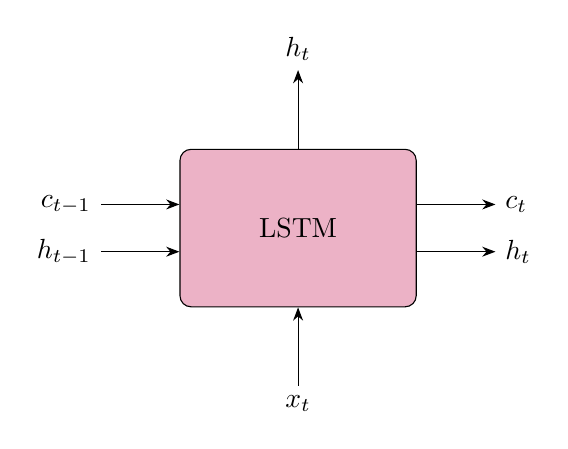
\begin{tikzpicture}[>=Stealth, node distance=1.5cm, auto]
  % LSTM cell as a pastel purple box with rounded corners
  \node[draw, fill=purple!30, rounded corners, minimum width=3cm, minimum height=2cm] (lstm) {LSTM};

  % Incoming arrows on the left: previous cell state (c) and hidden state (h)
  \draw[<-] ([yshift=0.3cm]lstm.west) -- ++(-1,0) node[left] {\(c_{t-1}\)};
  \draw[<-] ([yshift=-0.3cm]lstm.west) -- ++(-1,0) node[left] {\(h_{t-1}\)};

  % Outgoing arrows on the right: new cell state (c) and hidden state (h)
  \draw[->] ([yshift=0.3cm]lstm.east) -- ++(1,0) node[right] {\(c_t\)};
  \draw[->] ([yshift=-0.3cm]lstm.east) -- ++(1,0) node[right] {\(h_t\)};

  \draw[<-] (lstm.south) -- ++(0,-1) node[below] {\(x_t\)};
  \draw[->] (lstm.north) -- ++(0,1) node[above] {\(h_t\)};
\end{tikzpicture}
\caption{Simplified illustration of an \ac{lstm} layer}
\label{fig:lstm}
\end{figure}

As $c_t$ and $h_t$ are helpful when predicting future actions and states \cite{chung2024predictingfutureactionsreinforcement} when considering the \ac{drc} architecture, I hypothesize that the same holds when using a regular \ac{lstm} layer. See \cref{fig:lstm}.

\subsection{Frame Stacking}
Frame stacking in \ac{rl} is a technique used to provide an agent with temporal context when tasked with choosing an action by combining the previous $n$ observations into a single input to the policy. In some environments an observation at a single timestep isn't enough to capture the full state. In the case of autonomous vehicles a single observation might not have information on whether a car is standing still or in motion, and the velocity of a car is important to take into account when making an action.

If we have an observation space of 18, and we want to stack the previous 4 frames to feed into a fully connected input layer to a \ac{nn} we would insted of having the input $o_t$, where $o_t$ is a vector of size 18, we would instead get $$s_t = [o_t, o_{t-1}, o_{t-2}, o_{t-3}]$$ which is a $18\times4$ matrix, which we flatten into a single vector of size 72. If we instead of having a fully connected input layer, have a \ac{cnn} or another architecture that takes spatial context into consideration when processing an input, we would not flatten it.

Frame stacking does not give the \ac{nn} architecture memory, however it does provide the network with short term temporal context. I hypothesize that for event and state prediction for an agent, having information about previous observations and their transitions is helpful for predicting how the state will change in the future. In the case of autonomous vehicles its natural to assume that knowing the speed of which a vehicle has been moving will be relevant when trying to predict where it will be $n$ steps into the future.

\section{Statistical tests}
\label{sec:stat_meth}
In this section I will discuss the two statistical methods used in this thesis, the Students t-test and Confidence Intervals.

\subsection{Central Limit Theorem}
The two statistical tests we perform both assume the distribution is Gaussian. The central limit theorem states that any observed mean $\bar{x}$, which is what we perform t-tests on and confidence intervals for, will be drawn from a Gaussian distribution, even if the underlying distribution of $x$ is Gaussian\cite{clt}. This theorem is what lets us perform these test.

\subsection{Students t-test}
The null hypothesis chosen, $H_0$, is that the method provides no change in expected performance. To confirm that the difference in performance between baseline and our method is statistically significant I performed an independent one-tailed t-test, i.e. I calculated the likelihood that the increase in observed performance, or a higher increase in performance, happened by chance, and not because the true mean of the performance of the developed method is increased from baseline.

We bootstrapped the full dataset several times, i.e. created new datasets by sampling with replacement from the original datasets, and trained my prediction \acp{nn} 

on every dataset. From this we get a distribution of performances that we can use to perform a t-test and get a $p$-value. If this $p$-value is lower than a specified threshold value $\alpha$ I consider the result to be statistically significant. I set $\alpha = 0.05$.

Formally: 
$$
H_0: \mu = \mu_0
$$
where $\mu$ is the mean of the method i developed, and $\mu_0$ is the baseline mean.
$$
t = \frac{\bar{x} - \mu_0}{s/\sqrt{n}}
$$

where $\bar{x}$ is the mean of the samples for the method i developed, $s$ is the standard deviation for the samples in the population and $n$ is the size of the population.

For a right tailed t-test, which i use to measure whether the accuracy for event prediction has improved:
$$p = P(T \geq t) = \int_{t}^{\infty} f_T(u)\,du$$

and for a left tailed t-test, which i use to measure whether the error for state prediction has decreased:
$$p = P(T \leq t) = \int_{-\infty}^{t} f_T(u)\,du$$

$$\text{Reject } H\_0 \quad \text{if} \quad p < \alpha$$

\subsection{Confidence Interval}
The confidence interval is a statistical test to determine a range in which the true mean lies, around the observed mean, commonly used is 95\%, meaning that for an observed mean $\bar{x}$ we determine that the true mean $\mu$ has a 95\% likelihood of being in the range $(\bar{x}+ CI, \bar{x} - CI)$\cite{ci}.


A $(1-\alpha)$ confidence interval for the population mean \( \mu \) when the standard deviation \( \sigma \) is known is given by:
\[
CI = \bar{x} \pm z_{\frac{\alpha}{2}} \cdot \frac{\sigma}{\sqrt{n}},
\]
where $\bar{x}$ is the sample mean, $z_{\frac{\alpha}{2}}$ is the critical value from the standard normal distribution, $\sigma$ is the population standard deviation, and $n$ is the sample size. $z_{\frac{\alpha}{2}} = 1.96$ for $\alpha = 0.05$, which we have.

For cases when the true standard deviation, $\sigma$ is unknown, like we have, the sample standard deviation $s$ is used instead, the confidence interval is now calculated by:
\[
CI = \bar{x} \pm 1.96 \cdot \frac{s}{\sqrt{n}}
\]


\section{Environments}
\label{sec:env_meth}
For a better understanding of what state and event predictions refer to in my experiments, it is important to understand what type of environments the methods to extract states events are used in. In \cref{sec:simpl_env} we describe the Simple Spread environment and in \cref{sec:kaz_env} we describe the Knights Archers Zombies environment.

\subsection{Simple Spread}
\label{sec:simpl_env}
I used simple\_spread\_v3, the 3rd version of the environment. In the Simple Spread environment there are $n$ agents, and $n$ landmarks. Simple spread is a cooperative environment where the goal of an agent is for all the agents to reach a landmark, without colliding with the other agents. The agents are modeled as circles and the landmarks as dots. This environment was chosen partially for its simplicity, and the intuitive understanding of what features humans would consider important in such a setting. Developing our methods for this environment should also be relatively efficient due to the observation space of size 18, which is smaller than most other PettingZoo environments, and as such training the prediction \acp{nn} and calculation of feature importance is less computationally expensive. The global reward, $R_g$, is the negative total distance from each landmark to the closest agent measured with euclidean distance and the local reward, $R_l$, is $-1$ for every agent a given agent is colliding with.

Both continuous and discrete actions are available, I went with discrete. In the discrete action space each agent has the ability to idle, move up, move down, move left, or move right. I used $n=3$ and local ratio $0.5$, i.e. the reward, $R$, for an agent is $R = 0.5\times R_g + 0.5\times R_l$. See \cref{fig:simple_spread_env}

A critical state are states where the agents actions strongly impact returns. As returns are correlated with rewards a critical state is likely a state where agents might collide or make significant progress on getting closer to the landmark.

\begin{figure}[H]
    \centering
    \fbox{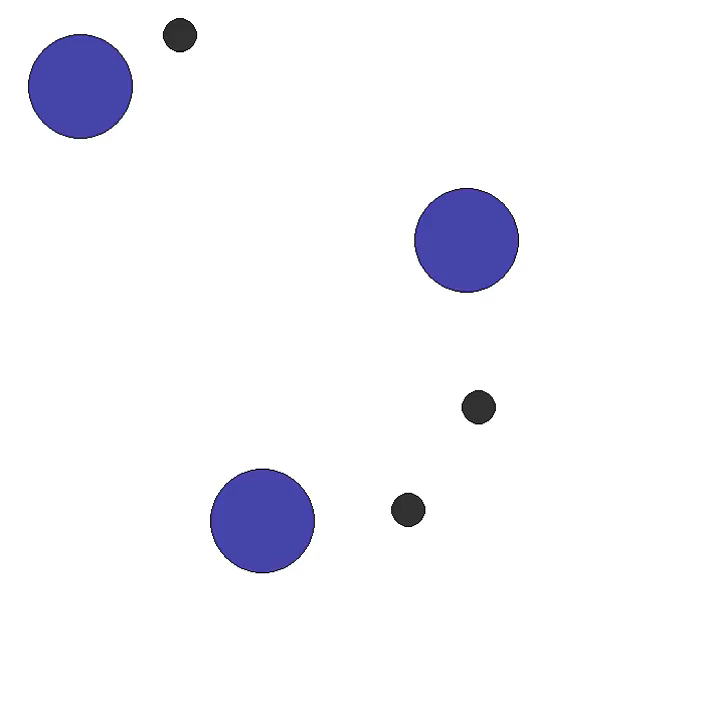
\includegraphics[scale=0.3]{images/simple_spread_v3/001.png}}
    \caption{Rendered frame from the Simple Spread environment. Agents are rendered as big blue circles, landmarks are rendered as small gray circles}
    \label{fig:simple_spread_env}
\end{figure}

\subsection{Knights Archers Zombies}
\label{sec:kaz_env}
I used knights\_archers\_zombies\_v10, the 10th version of the environment. The KAZ environment has a maximum of $n$ archers, a maximum of $m$ knights, and a maximum number of zombies $k$. The environment initializes with $n$ archers, $m$ knights and 0 zombies. The goal is for the archers and knights to kill zombies. Zombies spawn at the top border, at a set spawn rate, and travel down the screen moving randomly to the left or right. If an archer hits a zombie with an arrow it gets a reward of 1, and if a knight hits a zombie with a mace it gets a reward of 1. Once a zombie gets hit it dies. If a zombie collides with an agent the agent dies. The game ends once all agents are dead, a zombie reaches the bottom of the screen or some max length is reached.

For my experiments I used 2 archers, 2 knights, and a maximum of 10 zombies. The action space is discrete and allows the agents to idle, move forward, rotate clockwise, rotate counter clockwise, and attack. The observation space is either image based or vector based. I will use vector based for my experiments, which makes it a size of 135. See \cref{fig:kaz_env}

In the Knights Archers Zombies environment a critical state might be a state where an agent could die or is about to shoot an arrow that might kill a zombie, as these states are associated with changes in returns, immediate in the case of killing a zombie and delayed lower returns in the case of dying as an agent, as this does not incur a penalty, but it does make the agent unable to gain future rewards.

\begin{figure}[H]
    \centering
    \fbox{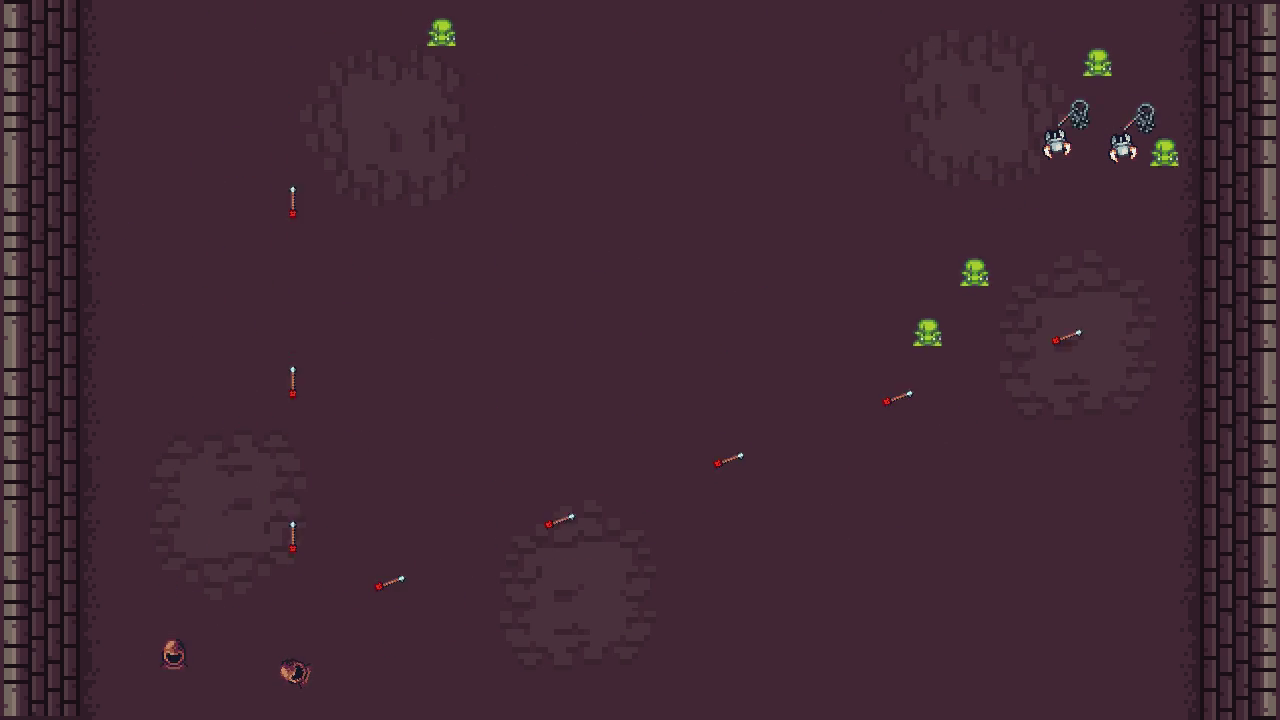
\includegraphics[scale=0.3]{images/knights_archers_zombies_v10/015.png}}
    \caption{Rendered frame from the Knights Archers Zombies environment.}
    \label{fig:kaz_env}
\end{figure}

\section{Policy creation}
This section will describe the details of how we create the policies for the environments.

\subsection{Reinforcement learning library}
There are a lot of options when deciding what library to use when designing \ac{rl} policies. I decided to use the library RLlib by Ray. The main benefits of this library is ease of implementation when working on heterogeneous agents, as each type of agent requires a specifically trained network to perform well. It also has scalability \cite{rayrllib}. It is required to train several policies for the creation of this thesis, therefore scalability when optimizing a policy is helpful.

\subsection{Policy construction}
I used a \ac{ppo} algorithm when optimizing my policy, because this method outperforms other algorithms in several environments in the continuous observation domain \cite{schulman2017proximalpolicyoptimizationalgorithms}, as well as the fact that is it applicable to \ac{marl} systems. The policy architecture consisted of an input layer with the observation of the environment as the size, two hidden layers of size 64, the hyperbolic tangent function, see \cref{eq:tanh}, colloquially known as tanh as the hidden layer activation function. This function is used for its "s-shape", bounding values from $y=-1$ to $y=1$, see \cref{fig:tanh}. The output layer has the size of the action space of the agent. For the \ac{lstm} policies I included a layer containing $64$ \ac{lstm} cells.

\begin{equation}
\label{eq:tanh}
tanh(x) = \frac{e^x-e^{-x}}{e^x+e^{-x}}
\end{equation}

\begin{figure}[H]
\centering
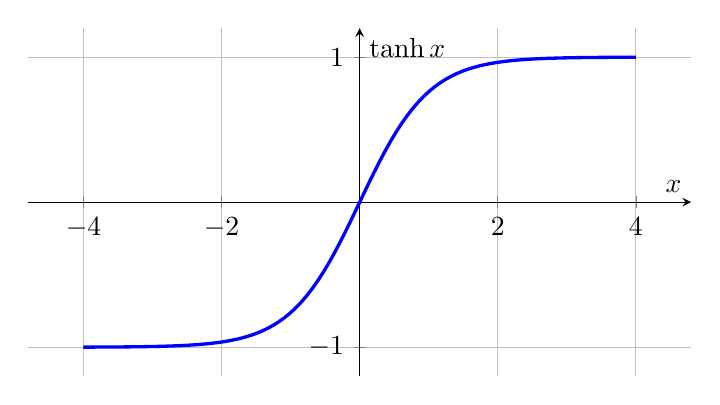
\begin{tikzpicture}
  \begin{axis}[
    xlabel={$x$},
    ylabel={$\tanh x$},
    domain=-4:4,
    samples=100,
    grid=both,
    axis lines=middle,
    width=10cm,
    height=6cm,
    enlargelimits,
  ]
    \addplot[blue, very thick] {tanh(x)};
  \end{axis}
\end{tikzpicture}
\caption{Graph showing the hyperbolic tangent function}
\label{fig:tanh}
\end{figure}

\subsection{Training}
The training was done with a batch size of 1024, for stability, $lr$ and $\gamma$ was automatically tuned for the policies in the Knights Archers Zombies environments, but in the Simple Spread environment I used $lr = 1e-4$ and $\gamma = 0.8$ s i found these to reach close to a global optimum for every variation of the environment I trained on, e.g. with or without frame stacking. The optimizer used was Adam as it outperforms other optimizers both for data efficiency and cost after convergence \cite{adam_optim}. The Adam optimizer calculates weights by computing the following equations:

\[
m_0 = 0, \quad v_0 = 0
\]

where $m_0$ and $v_0$ are initialized values.

\begin{equation*}
\begin{gathered}
  g_t = \nabla_{\theta} \pi_\theta(\theta_{t-1}) \\
  m_t = \beta_1 m_{t-1} + (1 - \beta_1) g_t \\
  v_t = \beta_2 v_{t-1} + (1 - \beta_2) g_t^2 \\
  \hat{m}_t = \frac{m_t}{1 - \beta_1^t} \\
  \hat{v}_t = \frac{v_t}{1 - \beta_2^t} \\
  \theta_t = \theta_{t-1} - \eta \, \frac{\hat{m}_t}{\sqrt{\hat{v}_t} + \epsilon}
\end{gathered}
\end{equation*}

where $g_t$ is the gradient of the policy error at timestep t, $m_t$ is the moving average of past gradients, $v_t$ is the moving average of past gradients squared. $\beta_1$ and $\beta_2$ are decay rates in the range $[0,1)$, $\hat m_1$ and $\hat v_2$ are bias corrected terms, and $\epsilon$ is a small constant for numerical stability. Since I will be using the gradients in the experiments, it is relevant to understand how the weights, which the gradients depend on, are created, and how these weights depend on the gradients as well.

\subsection{Softmax values}
After the policy has been created, for some experiments I append a softmax layer. The softmax layer is a common transformation to transform logits into likelihoods\cite{softmax}. The softmax function is defined as
\[
\sigma(\mathbf{z})_i = \frac{e^{z_i}}{\sum_{j=1}^K e^{z_j}},
\]
where \( \mathbf{z} = (z_1, z_2, \ldots, z_K) \) is a vector in \( \mathbb{R}^K \). I.e. if we have an action space $n=5$, then $K=5$. $\sigma(\mathbf{z})_i$ is the likelihood of action $i$. This transformation has the property of when summing across $i$, which also has $K$ different possible values, we always get $1$, which is to be expected since it represents a likelihood. This is a common trick to improve performance for \acp{nn} applications.

\section{Summary}
In short, this section describes what I will explore with the experiments.

\subsection{Event and state prediction}
I aim to predict event and state. The event I will predict are critical states, and the part of the state I will predict is future position. Critical states are defined as states with a high maximum logit difference. I will train \acp{nn} with auxiliary information to find what auxiliary information is most helpful to predict events and states. 

\subsection{Auxiliary information}
When predicting states and action I will include both actions and feature importance. The actions I include will be encoded as both integer and a one-hot vector. The feature importances will be attributed by using Integrated Gradients, or Shapley values. In total I will train 9 \ac{nn} in each case, one for each combination of action and explanation.

\subsection{Statistical test}
I will perform t-tests on the final performance of the \acp{nn} I have trained to discover whether the results are statistically significant, and I will otherwise perform confidence intervals for graphs.

\subsection{RL setup}
I will train a PPO algorithm in the simple spread environment, as well as the knights archers zombies environment, with small policies to perform the experiments on, after i use the policies trained to create datasets.

\chapter{Experiments}
\label{chap:exp}
This chapter will discuss the details on how i perform the experiments, as well as discussing and analyzing the results of these experiments. The experiment described in \cref{sec:exp_simpl} will be about detecting the effects of actions and feature importance and their ability to elucidate the intent of a policy as aforementioned, the experiments described in \cref{sec:exp_lstm} and \cref{sec:exp_stack} explores if and how temporal information can be used to explain the intent of a policy, and the experiments described in \cref{sec:exp_param} explores how to alter the event and state prediction networks to improve predictions.

\section{General experimental setup}
I have several \acp{nn} for each experiment. The \acp{nn} have two hidden layers of size 64 each, the activation function $tanh$, and outputs either part of the state, $(x,y)$ coordinates for an agent for state prediction, or a single value, whether the trajectory contains a critical state or not, for event prediction. The experiments attempt to test whether my developed methods have an effect on event and state predictions, how impactful these effects are and what contributes to whether the effect is significant or not.I trained them with a scheduler which would divide learning rate by $3$ from an original of $1e-4$, down to a minimum of $1e-6$ whenever the calculated loss on the validation set stopped decreasing. All training was stopped after 200 epochs.

\subsection{State prediction neural nets and datasets}
For the state prediction I initially trained a \ac{nn}, $state_{base}$ to take the observations made by a type of agent from step $n$, $Obs_n$, and output the $x$ and $y$ coordinates of the same agent at step $n+m$ in a trajectory. The dataset $D_{pos}$ was constructed such that each data point was from a different trajectory $\tau$, to make sure all the data points were independent of each other, in order to make sure the \ac{nn} did not learn any such connection. Each data point is a pairing of values $(Obs_n, (x_{n+m},y_{n+m}))$. The variable $n$ was chosen randomly for each trajectory while $m$ stayed as a constant, in my case $m=10$. I would for example have $50000$ trajectories, each trajectory contains $2$ archers, so we would have a dataset of size $100000$. $100000$ observations and their corresponding positions $10$ steps into the future. We assume that both archers use the same policy as they are homogeneous.

\subsection{Event prediction neural nets and datasets}
I also trained a \ac{nn} for event prediction, $event_{base}$. The event we trained a network to predict was whether an agent would encounter a critical state or not. See \cref{sec:event_state_meth}. The dataset $D_{crit}$ was similar to $D_{pos}$, however instead of positions, it would contain whether the agent would encounter a critical state within the next $4$ steps, $(Obs_n, crit)$, where $crit$ is a binary value, 0, for non critical states, or 1, for critical states.

I consider the accuracy of $event_{base}$ and the average error measured in euclidean distance of $state_{base}$ to be the baselines i compare results for including action against in the first experiment. I will train other \acp{nn} with different sets of auxiliary information as well, and compare the performance of these \acp{nn} to their baselines.


\subsection{Baseline performance}
$event_{base}$ and $state_{base}$ are as mentioned considered baselines for comparison for the \acp{nn} containing action in their input. The performances of these models will be located in the top right of all result tables. These \acp{nn} are purely post hoc explainers and used no information about the policy to explain the agents intention. As aforementioned we want to include information about the policy to discover how we can improve this prediction, and better discover the intent of the agent. For the \acp{nn} containing feature importance the baseline is considered to be the performance of the \ac{nn} without explanation, and with the corresponding action values. E.g. the baseline for the \ac{nn} with included action encoded as integer and Shapley values is the performance of the \ac{nn} with action included as integer but no explanation. The p-values marked is compared to their respective baselines.

Only The dataset, and therefore also the input layer, was different between the runs. I trained each network until improvement was negligible, for a maximum of 1000 epochs, which none of the networks reached, with a learning rate scheduler that decreased learning rate when loss reached a plateau, which was measured on a validation set. The scheduler divided learning rate by 3 each time more than 10 epochs had passed since last time it lowered learning rate and the loss had decreased by less than 0.0001. The learning rate had an initial value of 0.0001 and once the learning rate dropped below $10^{-6}$ I considered the training as stagnated.

\subsection{Action and explanation inclusion}
I enhanced both the dataset $D_{pos}$ and $D_{crit}$ with a series of other data. For both datasets I included the action, encoded by an integer from $0$ to $n_{acts}$, i.e. the amount of actions an agent has available, taken at $Obs_n$ for each data point, to use as input for an \ac{nn}. I then trained two \acp{nn} with the same architecture as $state_{base}$ and $event_{base}$ respectively, and once again measured accuracy for the event predictor net with included action, and average error for the state predictor net with included action. If the predictions improved I considered the action to be useful on its own for the predictions in the given environment.

This section will go into detail on how I included actions and explanations.

\subsubsection{One-hot and integer inclusion}
I then one-hot encoded the action, i.e. encoded the action as a $n_{acts}$ dimensional unit vector with a 1 in the chosen action dimension. This includes the same amount of information as represented as an integer, however I hypothesized that the resulting network would achieve higher performance with one-hot encoded actions as the distance between independent actions when one-hot encoding the actions are all the same, as opposed to when encoding the actions as an integer when the distance between two actions is not constant. For example, between the action encoded as the integer 2 and the action encoded as the integer 3 the Manhattan distance is 1, but between the action encoded as the integer 2 and the action encoded as the integer 4 the Manhattan distance is 2. When one-hot encoding these actions the Manhattan distance between two distinct actions will in all cases be 2. As in the previous cases I also trained a \ac{nn} on the datasets enhanced with one hot encoded actions.

\subsubsection{Integrated Gradients and Shapley Value inclusion}
After creating datasets with actions encoded different ways I also created two feature importance explanations for the action chosen in each of the initial observations. Shapley values and Integrated gradients were the two methods chosen. I decided on 2 feature importance measures that internally uses different methods of calculation, gradients and SHAP, to explore if they would yield different results. The motivation behind including feature importance explanations is that it describes some if the inner processing of the policy, and might therefore elucidate what kind of actions it might take in future states, and therefore include some of the intent. On each of the previous datasets I created new datasets with these two feature importance methods included.\\

\subsubsection{Softmaxing the policy output}
When softmaxing the output of the policy when computing Shapley Values and Integrated Gradients, the feature importances reflect what features were most influential to an agents confidence. If you do not softmax the output the feature attributions do not necessarily reflect confidence but rather better reflect the expectation og how good the chosen action is. Both of these could be useful when predicting future actions, so I will do both methods and analyze the results.

\subsection{Result presentation}
In total I trained 18 neural networks per policy, one for each dataset constructed, and compared the results for accuracy on the event prediction networks and the results for average error on the state prediction networks. I repeated this experiment for a few different environments and policies to explore if the results vary depending on environment or policy.

All results are presented in tables, with asterisks marking statistical significance, and italics used for baseline value.

\section{Simple Spread}
\label{sec:exp_simpl}
Here we will perform the experiments in the Simple Spread environment, first when softmaxing the policy, then without the softmax activation function, and then we will perform the experiment on a non-optimal policy.

\subsection{Setup}
The first experiment is divided into multiple subsections. First we will perform this experiment on a well trained policy on the simple spread environment, twice, first with softmaxed policy outputs for feature importance attribution, then without softmaxing the policy outputs. We will also observe the effects on event and state prediction when truncating training after reaching a decent policy performance but not as strong as in the first part of the experiment. For the sake of brevity I will only repeat the experiments with the highest increase in performance for the truncated training.

\subsection{Simple Spread with Softmax Activation}
All explainability methods in this section will refer to when explaining softmaxed outputs.


On state predictions for the Simple Spread environment, the inclusion of explanation methods are not shown to be an improvement over baseline. It is possible that in the case of predicting positions, the observation along with action is enough to predict future position, if the policy is close to optimal, or that correlations between explanations and actions, and future position is harder to learn, and would therefore require training time, or a larger network. I will investigate this further in this experiment as well as \cref{sec:exp_param}. See \cref{tab:state_simpl}.

\begin{center}
\captionof{table}{Average error for state prediction on the Simple Spread environment, mean over 10 computations}
\label{tab:state_simpl}
\begin{tabular}{lrrr}
\toprule
& No explanation & Integrated Gradients & Shapley Values \\
\midrule
No action & \textit{0.131317} & 0.133403 & 0.132936 \\
Integer & 0.129741 & 0.136067 & 0.131426 \\
One-hot & 0.123522*** & 0.128827 & 0.124774 \\
\bottomrule
\multicolumn{3}{l}{\textsuperscript{***}$p<0.001$, 
  \textsuperscript{**}$p<0.01$, 
  \textsuperscript{*}$p<0.05$}
\end{tabular}
\end{center}

When considering the event predictions for the Simple Spread environment the inclusion of explanations not not make a significant difference. The inclusion of action encoded as integer and as one-hot do reduce misclassifications by $1-\frac{1-0.717247}{1-0.704963} \approx 4.2\%$ and $1-\frac{1-0.737123}{1-0.704963} \approx 10.9\%$ respectively.

\begin{center}
\captionof{table}{Accuracy for event prediction on the Simple Spread environment, mean over 10 computations}
\label{tab:crit_simpl}
\begin{tabular}{lrrr}
\toprule
 & No explanation & Integrated Gradients & Shapley Value \\
 \midrule
    No action & \textit{0.704963} & 0.708020 & 0.689750 \\
Integer & 0.717247* & 0.704267 & 0.683190 \\
One-hot & 0.737123*** & 0.713717 & 0.723357 \\
\bottomrule
\multicolumn{3}{l}{\textsuperscript{***}$p<0.001$, 
  \textsuperscript{**}$p<0.01$, 
  \textsuperscript{*}$p<0.05$}
\end{tabular}
\end{center}

\subsection{Simple Spread without Softmax Activation}
\label{sec:simpl_no_sm}
All explainability methods in this section will refer to when the outputs of the policy \ac{nn} is not softmaxed.

On state prediction in the Simple Spread environment including explanations do not improve predictions. In all cases the observed accuracy gets meaningfully worse, which probably means in the case of future predictions, the explanations that are included require to be softmaxed for any meaningful improvement. It is worth to note that with sufficient training, and while avoiding overfitting, performance of the model after expanding the input should at most be equivalent to the unexpanded input model, as including more information makes it harder to distinguish relevant information, but does not decrease the quality or relevancy of relevant information. Softmaxing the output of the policy network can be considered normalization of feature importances so the value of one feature contains information on how important that feature is relatively to the complete explanation, which is not the case when not softmaxing the output of the policy as then the feature importances only paint a picture together, but contain less relevant information on their own. This is why it is not surprising to see performance drop when not softmaxing policy outputs. See \cref{tab:state_simpl_log}.

\begin{center}
\captionof{table}{Average error for state prediction on the Simple Spread environment without frame stacking, mean over 10 computations}
\label{tab:state_simpl_log}
\begin{tabular}{lrrr}
\toprule
 & No explanation & Integrated Gradients & Shapley Values \\
\midrule
No action & \textit{0.130958} & 0.145947 & 0.137418 \\
Integer & 0.130880 & 0.157760 & 0.137155 \\
One-hot & 0.123053*** & 0.155843 & 0.127923 \\
\bottomrule
\multicolumn{3}{l}{\textsuperscript{***}$p<0.001$, 
  \textsuperscript{**}$p<0.01$, 
  \textsuperscript{*}$p<0.05$}
\end{tabular}
\end{center}

For event prediction on the Simple Spread environment both including actions and explanations increase performance by a significant margin. Compared to the baseline accuracy the performance of the \ac{nn} when including one-hot encoded action without any explanation as input, the performance of the \ac{nn} when including Integrated Gradients without any action, as well as the performance of the combination of the two all increase by a significant margin, with the \ac{nn} with access of the combination of the two performing better than each of them did when included individually. The best performing network misclassified $1-0.705740 = 0.29426$ of instances, compared to $1-0.751387 = 0.248613$ the baseline, a decrease of $1-\frac{0.248613}{0.29426} = 0.155124 \approx 15\%$

It is worth to consider that there is a possible trivial correlation between including the feature importance for the maximum logit output, i.e. explanation for the chosen action, and whether the agent will encounter a critical state, as we consider states with high difference in maximum and minimum logit value as critical. Both integrated gradients, and Shapley values have the property of fully explaining the output from the features, i.e. the sum of the Integrated Gradients and the sum of the Shapley values both add up to the logit they are explaining. There is no direct correlation as the feature importance and explanation are from step $n = t$ in any given trajectory and the sub-trajectory considered is from step $n=t+1$ up to and including step $n=t+5$. I have not measured the correlation between the criticality of step $n$ and the criticality of the sub-directory considered, or the correlation between the maximum logit value in a state and the maximum logit difference in that state, so I do not know how impactful these are. Even in the extreme case of the entire increase in performance for included Shapley values is a direct result of this correlation, the increase in performance for included Integrated Gradients is meaningful compared to Shapley values, which reveals the fact that the correlations between critical states and explanations are not entirely trivial. This is confirmed by the fact that inclusion of Shapley values does not significantly improve predictions when also including one-hot values, but including Integrated gradients does significantly improve predictions.

\begin{center}
\captionof{table}{Average accuracy for event prediction on the Simple Spread environment, mean over 10 computations}
\label{tab:crit_simpl_log}
\begin{tabular}{lrrr}
\toprule
& No explanation & Integrated Gradients & Shapley values \\
\midrule
No action & \textit{0.705740} & 0.745593*** & 0.726290*** \\
Integer & 0.723123*** & 0.748297*** & 0.734843*** \\
One-hot & 0.738127*** & 0.751387*** & 0.730787 \\
\bottomrule
\multicolumn{3}{l}{\textsuperscript{***}$p<0.001$, 
  \textsuperscript{**}$p<0.01$, 
  \textsuperscript{*}$p<0.05$}
\end{tabular}
\end{center}


\subsection{Truncated training}
Before delving into the specifics of this experiment, I have chosen to perform the event prediction experiments with softmaxed policy outputs, and the state prediction experiments without softmaxed values on all future experiments.

In the case of state prediction on the Simple Spread environment, we get similar results to the case without truncated training, with the main difference being that we do not find statistical significance for improvement for the \ac{nn} with access to action encoded as integer.

\begin{center}
\captionof{table}{Average accuracy for event prediction on the Simple Spread environment, mean over 10 computations}
\label{tab:state_simpl_trunc}
\begin{tabular}{lrrr}
\toprule
& No explanation & Integrated Gradients & Shapley values \\
\midrule
No action & 0.128435 & 0.132283 & 0.129489 \\
Integer & 0.127049 & 0.132629 & 0.128414 \\
One-hot & 0.121558*** & 0.125370 & 0.122298 \\
\bottomrule
\multicolumn{3}{l}{\textsuperscript{***}$p<0.001$, 
  \textsuperscript{**}$p<0.01$, 
  \textsuperscript{*}$p<0.05$}
\end{tabular}
\end{center}


When looking at event prediction in the simple spread environment we can see that in the case of truncated training, whether the agent considers a state critical or not is easier to predict. In \cref{sec:mld} we discussed how an agents certainty about choosing an action affects whether that state is considered critical or not. When the agents policy is not trained to be optimal an agent sometimes pick a suboptimal action, that it eventually learns is suboptimal, in states like these it will eventually learn to be more certain about what action is preferable, as we know, because otherwise it would not improve. Eventually an agent is certain about what action to choose in every state, and in the previous experiment where this was the case, and the policy had converged, we can see that its harder for a neural network to differentiate between states with higher and lower certainty. The baseline performance for the similar case where the only difference is training time for the agent, and therefore also performance of the agent was an accuracy of $0.705740$ compared to this case with the baseline accuracy of $0.725047$. That is an decrease of misclassified states from $1-0.705740 = 0.29426$ to $1-0.725047 = 0.274953$, which is a $1-\frac{0.274953}{0.29426}=0.06561\approx 6.5\%$. We can see an increase in performance in all cases, albeit less pronounced in the cases with explanations. One reason for why inclusion of explanation does not see as high of an increase in performance is possible that either the distinguishing information present in the case with the truncated training that enables the baseline to perform better is also partially present in the explanations, or the performance seen by including explanations is strong enough to improving it in the Simple Spread environment, might need a greater change than training time to achieve significant improvements. See \cref{tab:event_simpl_trunc}.

\begin{center}
\captionof{table}{Accuracy for event prediction on the Simple Spread environment, with truncated training}
\label{tab:event_simpl_trunc}
\begin{tabular}{lrrr}
\toprule
 & No explanation & Integrated Gradients & Shapley Values \\
 \midrule
No action & \textit{0.725047} & 0.758307*** & 0.734053*** \\
Integer & 0.731497* & 0.761020*** & 0.741317** \\
One-hot & 0.752537*** & 0.759440*** & 0.736893 \\
\bottomrule
\multicolumn{3}{l}{\textsuperscript{***}$p<0.001$, 
  \textsuperscript{**}$p<0.01$, 
  \textsuperscript{*}$p<0.05$}
\end{tabular}
\end{center}

\subsection{Analysis}
In this section I will discuss the most interesting findings more in depth. I consider the most interesting findings to be when a correlation, other than trivial ones, were found.


When looking at a plot of the mean losses on a validation set during training we can see that the time each network takes to reach convergence varies wildly, at which point their training was truncated. I observed that when performing the experiments with a set number of epochs, some \acp{nn}, did not converge at all while some \acp{nn} converged a high number of epochs before reaching the set maximum, which was 400, and when learning rate starts to drop they all converge shortly after. All \acp{nn} with access to Integrated Gradients as input converged with fewer than 300 epochs, with Integrated Gradients and One-hot converging with the fewest required epochs, as well as reaching the best performance. Interestingly all \acp{nn} with access to any form of explanation converged significantly faster than any of the \acp{nn} that do not have access to explanations. Seeing as the best performing network without access to Integrated Gradients was the network with access to one-hot and feature importance input, it is likely that in this case adding Shapley values is about as helpful as adding noise. In the case of no action or action encoded as integer we do see improvements for the respective networks with Shapley included as well. See \cref{fig:crit_losses}.

\begin{figure}[H]
    \centering
    \import{images/simple_spread_v3/no_memory/agent}{crit_models_losses_plot_keep.pgf}
    \caption{Plot of losses during training of the event prediction networks on the Simple Spread environment, without softmaxing policy outputs.}
	\label{fig:crit_losses}
\end{figure}

No obvious patterns emerge when looking at the performance during training on the knights archers zombies environment. All the \acp{nn} stagnate at similar epochs and descend at a similar pace. This likely means the explanations do not contain information relevant to predicting future position for this policy and these prediction networks.

\begin{figure}[H]
    \centering
    \import{images/simple_spread_v3/no_memory/agent}{pred_models_losses_plot_keep.pgf}
    \caption{Loss on evaluation set for state prediction in the Simple Spread environment}
	\label{fig:pred_losses}
\end{figure}

\subsubsection{About the figures}
In all figures for feature value attribution on the event prediction and state prediction networks, only the 15 most influential features are included, to limit the size and density of the plots. It is natural to consider the features not included as not very influential for the predictions made.

I categorise the Shapley plots created into 2 types. One is plots where the observation is included and the second is the plots of shapley values of only the explanation. Even though these plots look similar, the colours of the samples represents 2 different things. For the plots with observations the colour of the samples represents high or low observation values, compared to other observation values, while in the plots without observations the colour represents the value compared to the value of other importances. To keep meanings of colours consistent in all plot, most feature values in the plots with observations will be represented with yellow, a value larger than the largest observation value.

\subsubsection{Event Prediction baseline}
For event prediction in the simple spread environment, we can see that the placement of the landmarks is gets the highest mean of feature attribution values for predicting whether an agent will encounter a critical state or not. Interestingly, with the exception of comms, which were turned off so they are expected to be irrelevant for predicting events, the features with the lowest attributed values were all current agent positions. Since the rewards are structured so that collisions between agents are penalized, it would be natural to expect that positions would be important when considering large differences in logits, that does however not seem to be the case, especially interesting is that the agents own position is the least influential factor when predicting whether the agent is about to encounter a critical state. Intuitively you could consider the position of the landmarks to be important as two landmarks in close proximity to each other might be challenging to reach by two separate agents without those agents colliding with each other. \cref{fig:event_simpl_shap} Shapley value attribution on one baseline event prediction \ac{nn}.


\begin{figure}[H]
\centering
\import{images/simple_spread_v3/no_memory/agent}{None_none_none_shap_keep.pgf}
\caption{Shapley Values on event prediction in the Simple Spread environment without included action or explanation. LM = Landmark, Vel = Velocity, Pos = Position.}
\label{fig:event_simpl_shap}
\end{figure}

\subsubsection{Event prediction with Integrated Gradients}
When including integrated gradients and action encoded as an integer for input to the event prediction networks, the Shapley values paint a picture of how influential the explanation especially is for the predictions. In \cref{fig:event_simpl_ig_shap} the Shapley values for the integrated gradients have been aggregated together to capture the importance of the entire explanation instead the influence of the explanation of each feature, which would be overshadowed by the observation of the agents importance. From the figure we can see that of the 50 instances plotted the explanation is, even in the case of the lowest Shapley value, more influential in predicting that the agent is about to encounter a critical state that any of the regular observations, even the instances with the highest attribution for regular observation values. This is not the case for predicting when the agent is not about to encounter a critical state, though the mean is still significantly more influential than the most influential instances of regular observations. Compared to the case in \cref{fig:event_simpl_shap} the variance in importance for observation features is reduced, and the order of the magnitudes seems arbitrary.

Looking at the Shapley diagram of the Integrated gradients separated from the rest of the inputs for the \acp{nn} without access to action, we can see that there very likely is a correlation between the feature value of the integrated gradients and the Shapley values, which I did consider as a possibility when performing the experiment, but to reiterate, that is not the only correlation between the integrated gradients and whether the following sub-trajectory contains a critical state. See \cref{fig:event_simpl_ig_slice}.

If we compare \cref{fig:event_simpl_ig_slice} to the Shapley diagram for the baseline network, \cref{fig:event_simpl_shap}, we see that the order of importance of observations correspond somewhat to the order of importance of integrated gradients. Beginning with landmarks, then the other agents, and then itself, with the exception of the importance of its own velocity, whose integrated gradients value is more important than observation value.
The velocity of itself for an agent is more important when including Integrated Gradients than otherwise, both the observation value and the integrated gradient value, though its likely that importance in state $s_t$ for event prediction in sub-trajectory $s_{t+1}$ to $s_{t+5}$ is correlated to importance for choosing an action in state $s_t$, which means its expected that the order of importance for the integrated gradients are correlated to the order of importance of the observation values, since the feature value of an integrated gradient value is correlated to importance.

If we take a look at the Shapley diagram for the best performing \ac{nn} for event prediction, the network with access to Integrated gradients and action encoded as one-hot, we observe that when aggregating one-hot Shapley values, they are the second most important component for predicting critical states. 

\begin{figure}[H]
    \centering
\import{images/simple_spread_v3/no_memory/agent}{None_none_ig_shap_keep.pgf}
\caption{Shapley Values on event prediction in the Simple Spread environment without included action, with Aggregated shapley values for Integrated Gradients explanations. IG = Integrated Gradients, LM = Landmark, Vel = Velocity, Pos = Position.}
\label{fig:event_simpl_ig_shap}
\end{figure}

\begin{figure}[H]
\centering
\import{images/simple_spread_v3/no_memory/agent}{None_none_ig_slice_shap_keep.pgf}
\caption{Shapley Values for Integrated Gradients, on event prediction in the Simple Spread environment, without including action. LM = Landmark, Vel = Velocity, Pos = Position.}
\label{fig:event_simpl_ig_slice}
\end{figure}

\begin{figure}[H]
    \centering
\import{images/simple_spread_v3/no_memory/agent}{None_one-hot_ig_shap.pgf}
\caption{Shapley Values for Integrated Gradients, on event prediction in the Simple Spread environment, with including action represented with a one-hot vector. LM = Landmark, Vel = Velocity, Pos = Position.}
\label{fig:event_simpl_one-hot_ig_shap}
\end{figure}

\begin{figure}[H]
    \centering
\import{images/simple_spread_v3/no_memory/agent}{None_one-hot_ig_slice_shap_keep.pgf}
\caption{Shapley Values for Integrated Gradients, on event prediction in the Simple Spread environment, with including action represented with a one-hot vector. LM = Landmark, Vel = Velocity, Pos = Position.}
\label{fig:event_simpl_one-hot_ig_slice}
\end{figure}

\subsubsection{State prediction baseline}
We can see from the Shapley diagram for state prediction on the Simple Spread environment that the baseline \ac{nn} acts intuitively. There is a strong correlation between all feature values of the observation and their Shapley values. This is likely partially due to the choice of what we want to predict, which I chose to be position. \cref{fig:state_simpl_shap} shows how influential each feature was for predicting the position along the $x$-axis, and as we can see from the diagram, all observation values related to $x$ position is more important than all observation values related to $y$ position, and very unsurprisingly, current position along the $x$-axis is the most important feature to predict future position along the $x$-axis.

This diagram likely highlights one reason why including Shapley values or Integrated Gradients did not improve the prediction. It highlights that if the agents acts rationally, the observation on its own is enough to predict future position. When including action encoded as one-hot value everything that is true for baseline is still the case. Aggregated one-hot values are less important that information about $x$-axis, but more important than information about the $y$-axis. See \cref{fig:state_simpl_one-hot}. When looking at the Shapley values for the \ac{nn} which includes Shapley values in the input this plot, \cref{fig:state_simpl_shap_shap} confirms there is not relevant information in the Shapley values that the \ac{nn} was able to extract, with the aggregated Shapley values being more important than nothing but pos x and pos y, as well as comms, but the comms always have zero importance.

When we find a correlation between feature values and Shapley values, where the features with correlations are the most influential ones, like we do in \cref{fig:event_simpl_ig_slice} and \cref{fig:state_simpl_shap}, we could train linear regression on the input. This would likely yield a decent result, would be inherently interpretable, and would drastically reduce training time. In these situations training a \ac{nn} is likely not optimal.

\begin{figure}[H]
    \centering
\import{images/simple_spread_v3/no_memory/agent}{0_none_none_shap_keep.pgf}
\caption{Shapley values for baseline state prediction in the simple spread environment for position along the $x$-axis. LM = Landmark, Vel = Velocity, Pos = Position.}
\label{fig:state_simpl_shap}
\end{figure}

\begin{figure}[H]
\centering
\import{images/simple_spread_v3/no_memory/agent}{0_one-hot_none_shap.pgf}
\caption{Shapley values for state prediction in the simple spread environment for position along the $x$-axis, with included action encoded as one-hot. LM = Landmark, Vel = Velocity, Pos = Position.}
\label{fig:state_simpl_one-hot}
\end{figure}

\begin{figure}[H]
\centering
\import{images/simple_spread_v3/no_memory/agent}{0_none_shap_shap.pgf}
\caption{Shapley values for state prediction in the simple spread environment for position along the $x$-axis, with included action encoded as one-hot. LM = Landmark, Vel = Velocity, Pos = Position.}
\label{fig:state_simpl_shap_shap}
\end{figure}

\section{Knights Archers Zombies}
In this section I will perform the experiments in the Knights Archers Zombies environment, first when using the knight as subject, then when using the archer.
\label{sec:exp_kaz}. As mentioned the state prediction network uses softmaxed output, and the event prediction network does not. Otherwise the setup is the same as in \cref{sec:exp_simpl}.

\subsection{Results for the Knights Archers Zombies environment}
First we will analyze the results when using Knights as a subject, then we will analyze the environment with focus on Archers. The knights archers zombies environment has an observation space of 135 in our case, compared to 18 in the simple spread environment. This might mean we need a wider \ac{nn} to properly extract relevant information, both for the policy and the prediction networks. This also means most of the Shapley values are not shown in the diagrams.

\subsection{Knights in the Knights Archers Zombies environment}

When looking at the results table for event prediction for knights in the knights archers zombies environment none of the additions made any significant difference. Interestingly one-hot encoding the action has been beneficial in every experiment so far, but makes no change in this case. See \cref{tab:event_kaz_knight}.

\begin{center}
\captionof{table}{Accuracy for event prediction on the Knights Archers Zombies environment, for Knights}
\label{tab:event_kaz_knight}
\begin{tabular}{lrrr}
\toprule
 & No explanation & Integrated Gradients & Shapley Values \\
\midrule
No action & \textit{0.817595} & 0.808390 & 0.792460 \\
Integer & 0.816145 & 0.807790 & 0.790675 \\
One-hot & 0.816690 & 0.808910 & 0.789370 \\ 
\bottomrule
\multicolumn{3}{l}{\textsuperscript{***}$p<0.001$, 
  \textsuperscript{**}$p<0.01$, 
  \textsuperscript{*}$p<0.05$}
\end{tabular}
\end{center}

From \cref{tab:state_kaz_knight} we can see that also in this case the inclusion of actions or explanations did not improve the performance on the knights archers zombies environment.

\begin{center}
\captionof{table}{Average error for state prediction on the Knights Archers Zombies environment, for Knights}
\label{tab:state_kaz_knight}
\begin{tabular}{lrrr}
\toprule
 & No explanation & Integrated Gradients & Shapley Values \\
\midrule
No action & \textit{0.033913} & 0.034564 & 0.035623 \\
Integer & 0.034292 & 0.034769 & 0.035554 \\
One-hot & 0.034618 & 0.034704 & 0.035322 \\
\bottomrule
\multicolumn{3}{l}{\textsuperscript{***}$p<0.001$, 
  \textsuperscript{**}$p<0.01$, 
  \textsuperscript{*}$p<0.05$}
\end{tabular}
\end{center}


\subsection{Archers in the Knights Archers Zombies environment}

In the case of state predictions on the Knights Archers Zombies environment for Archers, the inclusion of Integrated gradients are beneficial for state prediction. The inclusion of actions seem to have made an impact on the accuracy of the state prediction, though this decrease in error might just stem from learned knowledge of how an action changes the state, rather than knowledge of how to extract intent from an action. As mentioned the output of the policy is softmaxed for the Shapley values but not for integrated gradients, and this has been the first time I got statistically significant results for state prediction, so I will reattempt state prediction without softmaxing policy output. See \cref{tab:state_kaz}.

\begin{center}
\captionof{table}{Average error, euclidean distance, for state prediction on the Knights Archers Zombies environment}
\label{tab:state_kaz}
\begin{tabular}{lrrr}
\toprule
 & No explanation & Integrated Gradients & Shapley Values \\
\midrule
    No action & \textit{0.018424} & 0.017848*** & 0.018467 \\
Integer & 0.018196 & 0.017810*** & 0.018021 \\
One-hot & 0.017684*** & 0.017508 & 0.017582 \\
\bottomrule
\multicolumn{3}{l}{\textsuperscript{***}$p<0.001$, 
  \textsuperscript{**}$p<0.01$, 
  \textsuperscript{*}$p<0.05$}
\end{tabular}
\end{center}

When using the archer as the subject in the knights archers zombies environment we find that including Integrated Gradients once again improves the prediction in all cases for included action. Similarly to knights in this environment including action as Integer or One-hot did not improve significantly over baseline performance.significantly over baseline performance.

\begin{center}
\captionof{table}{Accuracy for event prediction on the Knights Archers Zombies environment, for Archers}
\label{tab:event_kaz_arch}
\begin{tabular}{lrrr}
\toprule
 & No explanation & Integrated Gradients & Shapley Values \\
\midrule
No action & \textit{0.754110} & 0.761055** & 0.722065 \\
Integer & 0.753495 & 0.760745*** & 0.722615 \\
One-hot & 0.754980 & 0.760970*** & 0.722590 \\
\bottomrule
\multicolumn{3}{l}{\textsuperscript{***}$p<0.001$, 
  \textsuperscript{**}$p<0.01$, 
  \textsuperscript{*}$p<0.05$}
\end{tabular}
\end{center}



\subsection{Analysis}
\subsubsection{Event Prediction for Knights}
The plot of losses on an evaluation set during training is interesting in the case of critical state prediction on the knights archers zombies environment for knights. There are three clearly distinct groups of lines, with similar sample efficiency, and similar performance. As in the Simple Spread environment, Shapley values for critical state prediction, had both lower sample efficiency, and lower final performance than Integrated Gradients. How the curves differ in this Environment is that both Integrated Gradients and Shapley Values seem to reach some local optimum that is different from the optimum found by the network when neither Shapley Values nor Integrated Gradients are included. The training time to reach stagnation is significantly longer than both with Shapley Values and Integrated Gradients, but it does not take too long, about 75 epochs to reach the performance of integrated gradients at epoch 50, to surpass Integrated Gradients in performance, and it has both higher data efficiency and better final performance than the \ac{nn} with access to Shapley values. See \cref{fig:event_knight_losses}.

\begin{figure}[H]
\centering
\import{images/knights_archers_zombies_v10/no_memory/knight}{crit_models_losses_plot.pgf}
\caption{Plot for loss measure on event prediction during training of 9 different neural networks,halfway opaque colour is confidence interval}
\label{fig:event_knight_losses}
\end{figure}

When looking at the Shapley Diagram of event prediction for knights in the knights archers zombies environment, \cref{fig:event_kaz_knight}, for the \ac{nn} with best observed performance, the baseline, it appears differently than most of the Shapley diagrams we have looked at so far. Here most features have Shapley values that seems to belong to one of two groups, where each group has similar feature value, with high variance between the groups and low variance within. The data efficiency for the \acp{nn} without included explanation is significantly higher in the knights archers zombies environment than in the simple spread environment. It is possible that these fact that the Shapley diagram appears with these groups is related to the fact that the data efficiency is so different.

In the simple spread environment we observed that when truncating training before reaching an optimal policy the accuracy for event prediction, when not including explanations increased compared to the optimal policy, but including Shapley values and Integrated gradients reached similar performance. A similar effect could be happening here, where a policy network with two hidden layers of size 64 is too small to reach close to optimal performance, and therefore get a better performance without explanations. It is also possible that Integrated Gradients and Shapley Values dont contain information that is not already present in the observation, just on a format that is simpler to extract for a \ac{nn}.

When looking at the Shapley diagram for the \ac{nn} with access to Integrated Gradients we can see that the Integrated Gradients are important for prediction. As this \ac{nn} converged faster than the \acp{nn} without included explanations, it is not surprising that these values are also more important for the final performance. The regular observation values still have this tendency to split into two groups when measuring importance. See \cref{fig:event_kaz_knight_ig}. When looking at the Shapley values for the Integrated Gradients separately they do not display the same correlation we observed for the simple spread environment, with higher feature values being correlated with higher Shapley values. It is possible that with some type of transfer training, where we introduce explanations gradually as it trains, we could leverage the explanations to improve on the predictions made without explanations. See \cref{fig:event_kaz_knight_ig_slice}.

\begin{figure}[H]
\centering
\import{images/knights_archers_zombies_v10/no_memory/knight}{None_none_none_shap.pgf}
\caption{Shapley values for state prediction in the simple spread environment for position along the $x$-axis, with included action encoded as one-hot. LM = Landmark, Vel = Velocity, Pos = Position.}
\label{fig:event_kaz_knight}
\end{figure}

\begin{figure}[H]
\centering
\import{images/knights_archers_zombies_v10/no_memory/knight}{None_none_ig_shap.pgf}
\caption{Shapley values for state prediction in the simple spread environment for position along the $x$-axis, with included action encoded as one-hot. LM = Landmark, Vel = Velocity, Pos = Position.}
\label{fig:event_kaz_knight_ig}
\end{figure}

\begin{figure}[H]
\centering
\import{images/knights_archers_zombies_v10/no_memory/knight}{None_none_ig_slice_shap.pgf}
\caption{Shapley values for state prediction in the simple spread environment for position along the $x$-axis, with included action encoded as one-hot. LM = Landmark, Vel = Velocity, Pos = Position.}
\label{fig:event_kaz_knight_ig_slice}
\end{figure}


\subsubsection{State Prediction for Knights}
When looking at the plot of losses in the case of predicting future position for knights in the knights archers zombies environment, it looks like all the observed means of \ac{nn} performance are within the confidence intervals of every other observed mean of performance, meaning that any observed difference is not significant and the networks did not manage to find any meaningful data in the auxiliary information provided. See \cref{fig:state_knight_losses}.

Because the confidence intervals are so high, its possible that with more runs we would find some statistical difference. There are methods to try to reduce this CI when training, a high CI is undesirable in cases where we want a random sample to be predictable, as we would in a practical application of future prediction. There are several potential causes and remedies to lower the CI observed. 

Since we see the curves diverge early it is possible that state prediction for knights is sensitive to weights initialization, and using another type of initialization might make early training robust to this divergence. All the weights for the \acp{nn} I have trained were initialized from a random uniform distribution. If I instead used a normal distribution, like normal Xavier initialization, we could avoid the problem of early exploding or vanishing gradients\cite{xavier_init}.

Another culprit might be that a large initial $LR$s changes the weights enough to jump into different valleys in the loss landscape, and the exploration isnt high enough to discover other, possibly deeper, valleys. It is also possible that the different bootstrapped datasets are not representative, but given the amount of samples of $100000$ which is enough to avoid overfitting in every other experiment, which are usually quite similar, I think this is unlikely.

\begin{figure}[H]
\centering
\import{images/knights_archers_zombies_v10/no_memory/knight}{pred_models_losses_plot.pgf}
\caption{Plot for loss measure on state prediction during training of 9 different neural networks, translucent colour is confidence interval}
\label{fig:state_knight_losses}
\end{figure}

\subsubsection{Event Prediction for Archers}

In the case of event prediction for Archers, the plots of the loss curves during training when not including integrated gradients looks similar to the corresponding plot for knights, except for the fact that the observation, and possibly Shapley values, contain less information about whether the agent is about to encounter a critical state that the \ac{nn} is able to extract. Including Integrated Gradients seems to improve predictions however. We have not found that including actions improves performance in this case either. See \cref{fig:event_archer_losses}.

\begin{figure}[H]
\centering
\import{images/knights_archers_zombies_v10/no_memory/archer}{crit_models_losses_plot.pgf}
\caption{Plot for loss measure on state prediction during training of 9 different neural networks, translucent colour is confidence interval}
\label{fig:event_archer_losses}
\end{figure}

There are several reasons for it might be the case that Integrated Gradients are beneficial for archers and not knights. In all cases where Integrated Gradients have improved predictions the accuracy of the \acp{nn} arrived at approximately $75\%$. See \cref{tab:crit_simpl_log}, \cref{tab:event_simpl_trunc}, \cref{tab:event_kaz_arch}. It is possible that Integrated Gradients along with the observation is often enough to get predictions to approximately $75\%$, but does not help after that.

The improvement in performance is relatively small, and from the loss curves it may seem that the training for no included explanation happens so similarly to the integrated gradients inclusion that an assumption one could make is that the Integrated Gradients help, but are not important to predictions. If we look at \cref{fig:event_archer_ig_shap}, we can see however, that this is not the case.

Even though the performances of the different \acp{nn} are similar between simple spread environment and knights archers zombies environment are similar, and the loss curves for no included action but included IG are similar, except for the fact that it converges faster in the KAZ environment, the Shapley plot for the integrated gradients is very different. As a reminder, \cref{fig:event_simpl_ig_slice}, had a seemingly positive linear correlation between feature values and Shapley values, \cref{fig:event_archer_ig_slice} does not display this, which suggests that the trivial correlation described in \cref{sec:simpl_no_sm} is not the correlation which improves performance.

\begin{figure}[H]
\centering
\import{images/knights_archers_zombies_v10/no_memory/archer}{None_none_ig_shap.pgf}
\caption{Shapley values for event prediction in the Knights Archers Zombies environment, with included Integrated Gradients.}
\label{fig:event_archer_ig_shap}
\end{figure}

\begin{figure}[H]
\centering
\import{images/knights_archers_zombies_v10/no_memory/archer}{None_none_ig_slice_shap.pgf}
\caption{Shapley values of Integrated Gradients for event prediction in the Knights Archers Zombies environment.}
\label{fig:event_archer_ig_slice}
\end{figure}

% \begin{figure}[H]
% \centering
% \import{images/knights_archers_zombies_v10/no_memory/archer}{None_none_none_shap.pgf}
% \caption{Shapley values for baseline event prediction in the Knights Archers Zombies environment.}
% \label{fig:event_archer_none_shap}
% \end{figure}


\subsubsection{State Prediction for Archers}

The plot of losses for state prediction on the Knights Archers Zombies environment, \cref{fig:state_archer_losses}, shows that the training for all 9 datasets are similar to each other, with similar data efficiency and similar performance. Barely visible on the plots are confidence intervals, because they are very slim. As we saw in table \cref{tab:state_kaz} we know that the increases in performance when including One-hot with no explanation (pink), no action and Integrated Gradients (orange) and action encoded as integer with integrated gradients (purple) are all highly statistically significant. Comparing this to \cref{fig:state_knight_losses} we can observe that in the same environment, predicting the same element of the state could yield different results. While performance and sample efficiency are similar for the 9 \acp{nn} trained for knights, the relative confidence intervals for knights were the highest we have measured so far, compared to for archers where they are the lowest.


\begin{figure}[H]
\centering
\import{images/knights_archers_zombies_v10/no_memory/archer}{pred_models_losses_plot.pgf}
\caption{Plot for loss measure on state prediction during training of 9 different neural networks, translucent colour is confidence interval}
\label{fig:state_archer_losses}
\end{figure}

In this thesis $x$-position refers to lateral position, and $y$-position refers to longitudinal position, $y=0$ is where zombies spawn, and $y=1$ is where the episode ends if a zombie reaches it, in the rendered environment. See \cref{kaz_env}.

If we look at the diagram of Shapley values for predicting $x$-position in the Knights Archers Zombies environment, \cref{fig:state_archer_ig_shap_0}, when including Integrated Gradients, their aggregated values do not show up among the 15 most important values, meaning that they are not important for predicting but are useful for making small adjustments to the prediction. Compared to the Shapley diagrams for event prediction when Integrated Gradients always show up as most important. Its likely that integrated gradients on their own is not enough to predict position well, at least for a small \acp{nn}, but is enough to predict critical states.

When looking at the Shapley values of the Integrated Gradients disaggregated, we can see that none of them have a very high impact on prediction. In this case we can see that the integrated gradients for arrows and self are more beneficial to performance than others, as out of the top 15 Shapley values, 11 of them refers to arrows, though all of them have low values and usually lie in the range $(-0.004, 0.004)$. See \cref{fig:state_archer_ig_slice_0}. 

If we instead look at the diagram of Shapley values for predicting $y$-position, the aggregated Integrated Gradients do show up among the top 15 features, as the 13th most important, out of 136. See \cref{fig:state_archer_ig_shap_1}.

When we disaggregate these values we see that also for $y$-position, out of the top 15 values, arrows account for 11 of them. Integrated Gradients are more beneficial when looking at $y$-position, which may mean the agent cares more about $y$-position than $x$-position, so the Integrated Gradients carry more information about future $y$-position, than future $x$-position. But also in this case are they not very impactful, usually ranging between $(-0.015,0.01)$.

\begin{figure}[H]
\centering
\import{images/knights_archers_zombies_v10/no_memory/archer}{0_none_ig_shap.pgf}
\caption{Shapley values for $x$-position prediction in the Knights Archers Zombies environment, with included Integrated Gradients.}
\label{fig:state_archer_ig_shap_0}
\end{figure}

\begin{figure}[H]
\centering
\import{images/knights_archers_zombies_v10/no_memory/archer}{0_none_ig_slice_shap.pgf}
\caption{Shapley values for $x$-position prediction in the Knights Archers Zombies environment, only Integrated Gradients.}
\label{fig:state_archer_ig_slice_0}
\end{figure}

\begin{figure}[H]
\centering
\import{images/knights_archers_zombies_v10/no_memory/archer}{1_none_ig_shap.pgf}
\caption{Shapley values for $y$-position prediction in the Knights Archers Zombies environment, with included Integrated Gradients.}
\label{fig:state_archer_ig_shap_1}
\end{figure}

\begin{figure}[H]
\centering
\import{images/knights_archers_zombies_v10/no_memory/archer}{1_none_ig_slice_shap.pgf}
\caption{Shapley values for $y$-position prediction in the Knights Archers Zombies environment, only Integrated Gradients.}
\label{fig:state_archer_ig_slice_shap_1}
\end{figure}


\section{LSTM hidden values and cell states inclusion}
\label{sec:exp_lstm}
In this experiment I will include \ac{lstm} hidden values and cell states, $(h,c)$ and observe the effects on performance as well including explanations and exploring how the effects differ in experiment from the experiment in \cref{sec:exp_simpl}.

\subsection{Setup}
There are two main ways of including temporal information in reinforcement learning policies. The first is to include more than just the last observation as input, known as frame stacking. Another design I implemented, that also includes temporal information for the policy is a design that includes an \ac{lstm} layer in that takes input from the second hidden layer and outputs to the last fully connected layer.

We once again construct datasets which contain pairs on the form $(obs, pos)$ and $(obs, crit)$ respectively. For the observations for the policy using an \ac{lstm} we also include the hidden values and cell states, $(h,c)$, as part of the input for the event prediction and state prediction \acp{nn}, to include the temporal information used by the policy for the prediction \acp{nn}, similarly to in the case with frame stacking.

\subsection{Actions and explanations}
I will once again include actions and explanations for the \ac{lstm} networks to observe the effect in this case. We observed in experiment one that actions encoded as one-hot vectors were more beneficial to the performance of the models than actions encoded as integers. We will therefore not include integers in this experiment and onwards.

The same applies to the explanations. For event predictions Integrated Gradients performed better, and for state prediction Shapley values performed better. Therefore I will not include Shapley values for event prediction or integrated gradients for state prediction in this experiment and onwards.

\subsection{Results}
I will first discuss the results when performing this experiment in the Simple Spread environment, and then in the Knights Archers Zombies environment, for both knights and archers. Presentation will be similar to the first experiment.

\subsubsection{Simple Spread}

\begin{center}
\captionof{table}{Average error for state prediction on the Simple Spread environment with \ac{lstm} output and cell states}
\label{tab:state_simpl_lstm}
\begin{tabular}{lrrr}
\toprule
 & No explanation & Integrated Gradients & Shapley Value \\
\midrule
No action & 0.306358 & 0.304827 & 0.305336 \\
Integer & 0.306486 & 0.304529 & 0.306255 \\
One-hot & 0.307398 & 0.305968 & 0.305619 \\
\bottomrule
\end{tabular}
\end{center}

\begin{center}
\captionof{table}{Average accuracy for event prediction on the Simple Spread environment with \ac{lstm} output and cell states}
\label{tab:event_simpl_lstm}
\begin{tabular}{lrrr}
\toprule
 & No explanation & Integrated Gradients & Shapley Values \\
\midrule
No action & 0.730967 & 0.775767 & 0.739200 \\
Integer & 0.715100 & 0.778400 & 0.741933 \\
One-hot & 0.728867 & 0.779600 & 0.742567 \\
\bottomrule
\end{tabular}
\end{center}

\subsubsection{Knights Archers Zombies}


\subsection{Analysis}


\section{Frame Stacking}
\label{sec:exp_stack}
The other way I considered adding temporal information was frame stacking. In this experiment I will explore the effects of frame stacking for event and state prediction, first on the simple spread environment, and then on the knights archers zombies environment. 

\subsection{Setup}
As discussed in \cref{sec:exp_simpl}, I will be using softmaxed policy outputs when exploring state prediction, and I will not be using softmaxed policy outputs when exploring event prediction.

\subsection{Results}
The results for this experiment will be divided into \cref{sec:simpl_exp3} for results on the simple spread environment and \cref{sec:kaz_exp3} for the knights archers zombies environment.

\subsubsection{Simple Spread}
\label{sec:simpl_exp3}
When we include frame stacking in the Simple Spread environment in our case we include the previous 3 observations as well so the total observation space has size $18\times 4 = 72$. This auxiliary information requires a new policy to be trained as the representation of the environment is different from the case without frame stacking. The baseline results are unchanged from the case without frame stacking, and all other improvements are less pronounced. See \cref{tab:state_simpl_stack}.

\begin{center}
\captionof{table}{Average error for state prediction on the Simple Spread environment with frame stacking}
\label{tab:state_simpl_stack}
\begin{tabular}{lrrr}
\toprule
 & No explanation & Integrated Gradients & Shapley Values \\
\midrule
No action & 0.303008 & 0.304275 & 0.298301 \\
Integer & 0.289100 & 0.305222 & 0.291256 \\
One-hot & 0.305099 & 0.305001 & 0.298962 \\
\bottomrule
\end{tabular}
\end{center}

For event prediction on the Simple Spread environment with frame stacking the results are improved for no explanation included, and improved in some cases when considering explanations as well, from the results in the case without frame stacking. See \cref{tab:event_simpl_stack}.

\begin{center}
\captionof{table}{Average accuracy for event prediction on the Simple Spread environment with frame stacking}
\label{tab:event_simpl_stack}
\begin{tabular}{lrrr}
\toprule
 & No explanation & Integrated Gradients & Shapley Values \\
\midrule
No action & 0.737900 & 0.80300 & 0.756633 \\
Integer & 0.724767 & 0.804433 & 0.763100 \\
One-hot & 0.766567 & 0.812067 & 0.780700 \\
\bottomrule
\end{tabular}
\end{center}

\subsubsection{Archers in Knights Archers Zombies}
\label{sec:kaz_exp3}

\subsubsection{Knights in Knights Archers Zombies}
\subsection{Analysis}


\section{Hyperparameter Exploration}
\label{sec:exp_param}
In this experiment i will review some of the earlier experiments with a larger state and event prediction network. This exploration will reveal if there is relevant information in the auxiliary information included in the experiments in \cref{sec:exp_simpl} through \cref{sec:exp_stack}. Though I will not repeat all experiments as training time would increase to an unreasonable amount of time in total if we were to retrain every single network.

\subsection{Setup}
First we will reduce network size to containing 2 hidden layers with only 32 nodes in each layer, as opposed to 64 nodes in each layer in earlier experiments, and repeat the experiments where auxiliary information improved performance on event and state prediction.

Then we will expand network size to containing 3 hidden layers, of size 128 each and repeat some of the experiments where we did not manage to improve performance to see the effects of a larger network size. If we do find significant improvement with a larger network size, it is likely that some of the auxiliary information does contain relevant information, but a network size with 2 hidden layers of size 64 each is too simple to meaningfully extract some of the information found in the more complex auxiliary information, like hidden and cell states.

\subsection{Results}


\subsubsection{Smaller network}


\subsubsection{Larger network}


\subsection{Analysis}



\chapter{Discussion}
\label{chap:disc}
In this chapter I will consider the limitations of my methods and future work that could be done to improve my methods or discover other interesting results.

\section{Limitations}
Due to the mainly theoretical nature of my work there are several components which restrict applicability to real world settings. We will discuss these as well as other limitations in this section.

\subsection{Explainability methods}
I only performed experiments with the feature importance methods SHAP and Integrated Gradients. In several experiments I observed significant differences in how these methods impacted the performance of the event and state prediction \acp{nn}, and it is very possible that there are other feature attribution methods that perform better, as well as other explainability methods all together, that outperform the methods explored in this thesis.

\subsection{Network size and construction}
Because we are exclusively working with fully connected networks with at most 3 hidden layers of 128 nodes each it is very possible that the results found here are not applicable to scenarios with larger network sizes. The methods developed could both be improved by larger network sizes, or the results could be diminished. It is for example possible that for a larger network size, observation on its own is enough to predict whether an agent is about to encounter a critical state or not. 
Another limitation is the size of the policy network, as the size of the policy network dictates how long it takes to compute integrated gradients, as well as Shapley values when using the method introduced by,  . Some real world scenarios will be time sensitive enough and have complex enough environments that the necessary policy size to perform well is large enough that calculating Shapley values or Integrated Gradients during inference is not feasible, especially if hardware constraints also are present. In these scenarios my methods will likely not be applicable.
Additionally, if a policy is not

\section{Future work}
In the example of autonomous vehicles, it is likely that a policy network with the same size I have worked with, i.e. 2 hidden layers of size 64 each, is not complex enough to capture the necessary correlations to drive a vehicle well. The correlations here are likely more complex than the correlations necessary to pilot the agents i have worked with well, and these correlations likely affect the performance of predicting future states and events with my methods. It is necessary to test all of these methods with larger policies and larger prediction networks in more complex environments to ascertain whether these methods are useful for applications other than theoretical research. 

\section{Explainable Reinforcement Learning Evaluation}
This section will describe how well the prediction \acp{nn} I developed fulfill some important criteria used to measure explanations. I will rank these on a scale low/medium/high, as formal tests do not exist for all of these, and are outside the scope of this thesis. Several of these measures are also subjective.

\subsection{Core criteria}
These are the criteria that do not relate to how a human understands the explanation but rather how an expert might rank it.

\subsubsection{Fidelity}
Fidelity is a measure of how close an explanation is to the reasoning of an underlying model. In our case the explanation is the event and state prediction \acp{nn}, and the underlying model is the policy of an agent. Since our explanation does little to elucidate how the policy manifests intent, and the explanation itself which are the event and prediction \acp{nn} and their outputs are not interpretable, though I do clarify what features the prediction \acp{nn} use to make their prediction with the Shapley Value plots. The fidelity of these explanations get a score of low.

\subsubsection{Stability}
Stability is a measure of how much the explanation changes when the input is slightly perturbed. I have not measured the stability, however as the prediction \acp{nn} do not overfit, the stability is likely to stay be high, as the domain is continuous, and slight perturbations are likely to keep the inputs in distribution.

\subsubsection{Faithfulness}
Faithfulness is a measure of how well the explanations identify influential features. This is related to fidelity, but curtains to features instead of reasoning. The faithfulness is hard to measure without a high fidelity explanation, but its not unreasonable to think that the faithfulness is high, seeing as similar features get similar Shapley Values.


\subsubsection{Consistency}
TO-DO explore whether similar models behave similarly.

\subsubsection{Completeness}
Completeness describes whether the explanation covers all aspects of the models reasoning, and not just a subset of features. Seeing as we do use the entire observation of the policy, the output of the policy and the feature importances of the observations, my explanation gets a score of medium. Feature importance is not enough to describe the reasoning of the model, and as such we are missing essential components for a high completeness explanation.

\subsection{Human related criteria}
These are the criteria related to how useful this explanation is when confronted by a layman.

\subsubsection{Interpretability}
Interpretability refers to how well understandable an explanation is. The methods outputs a future prediction, along with feature importances that lead to the given prediction. It tells what will happen and how do we know. Though it does not elucidate the connection between what is important to know to make the prediction, and the prediction itself. It receives a score of medium.

\subsubsection{Comprehensibility}
Comprehensibility relates to how easily a human can understand the explanation. These methods are very comprehensible, the methods tell you an agent "wants" to go here or it "thinks" x will happen. An agent of course has neither wants nor thoughts, but to a layman, an explanation about what the agent wants to achieve can explain a range of actions prior to the expected consequence. These methods score high on comprehensibility. This is related to interpretability. An example that clearly explains the difference is a diagram of a car. It might be very interpretable, but could take time or prior knowledge to understand, which lowers comprehensibility.

\subsubsection{Simplicity}
Refers to how well the explanations fit into a persons reasoning process, or working memory. An explanation like "this car is about to take a right turn, because of the fractional influence of 67 superpixels" is a low simplicity explanation. I have attempted to increase simplicity by sorting influential features into categories of similar features, to increase simplicity from low, to a medium. 

\subsubsection{Actionability}
Actionability refers to whether the explanation impacts the users ability to take action, such as fixing a model, or take over control. In my case this is often an ability the user has. An explanation like "this vehicle is about to encounter a high risk state" gives the user the ability to take over control if they believe they are better at managing the high risk state than the car is. It also gives the user the ability to take over if the vehicle decides to take a detour without a rational explanation for why. Alternatively you could investigate further to find out what kind of states are viewed as high risk and modify the agent to perform better in these states. The actionability of future prediction methods are high.

\subsubsection{Trustworthiness}
Trustworthiness reflects whether an explainability method promotes trust, or distrust, in a system. Future state and event prediction are two of the most important factors when deciding whether an agent is acting reasonably, and therefore promotes appropriate trust. The trustworthiness is therefore high.


\cite{chung2024predictingfutureactionsreinforcement}

\section{Summary}

\appendix

\chapter{Diagrams}
In appendix A are all diagrams that are referred to, but not necessary to see to keep up with the analysis of the experiments or otherwise.


\printbibliography{}
\end{document}
